\documentclass[11pt]{article}

    \usepackage[breakable]{tcolorbox}
    \usepackage{parskip} % Stop auto-indenting (to mimic markdown behaviour)
    

    % Basic figure setup, for now with no caption control since it's done
    % automatically by Pandoc (which extracts ![](path) syntax from Markdown).
    \usepackage{graphicx}
    % Maintain compatibility with old templates. Remove in nbconvert 6.0
    \let\Oldincludegraphics\includegraphics
    % Ensure that by default, figures have no caption (until we provide a
    % proper Figure object with a Caption API and a way to capture that
    % in the conversion process - todo).
    \usepackage{caption}
    \DeclareCaptionFormat{nocaption}{}
    \captionsetup{format=nocaption,aboveskip=0pt,belowskip=0pt}

    \usepackage{float}
    \floatplacement{figure}{H} % forces figures to be placed at the correct location
    \usepackage{xcolor} % Allow colors to be defined
    \usepackage{enumerate} % Needed for markdown enumerations to work
    \usepackage{geometry} % Used to adjust the document margins
    \usepackage{amsmath} % Equations
    \usepackage{amssymb} % Equations
    \usepackage{textcomp} % defines textquotesingle
    % Hack from http://tex.stackexchange.com/a/47451/13684:
    \AtBeginDocument{%
        \def\PYZsq{\textquotesingle}% Upright quotes in Pygmentized code
    }
    \usepackage{upquote} % Upright quotes for verbatim code
    \usepackage{eurosym} % defines \euro

    \usepackage{iftex}
    \ifPDFTeX
        \usepackage[T1]{fontenc}
        \IfFileExists{alphabeta.sty}{
              \usepackage{alphabeta}
          }{
              \usepackage[mathletters]{ucs}
              \usepackage[utf8x]{inputenc}
          }
    \else
        \usepackage{fontspec}
        \usepackage{unicode-math}
    \fi

    \usepackage{fancyvrb} % verbatim replacement that allows latex
    \usepackage{grffile} % extends the file name processing of package graphics
                         % to support a larger range
    \makeatletter % fix for old versions of grffile with XeLaTeX
    \@ifpackagelater{grffile}{2019/11/01}
    {
      % Do nothing on new versions
    }
    {
      \def\Gread@@xetex#1{%
        \IfFileExists{"\Gin@base".bb}%
        {\Gread@eps{\Gin@base.bb}}%
        {\Gread@@xetex@aux#1}%
      }
    }
    \makeatother
    \usepackage[Export]{adjustbox} % Used to constrain images to a maximum size
    \adjustboxset{max size={0.9\linewidth}{0.9\paperheight}}

    % The hyperref package gives us a pdf with properly built
    % internal navigation ('pdf bookmarks' for the table of contents,
    % internal cross-reference links, web links for URLs, etc.)
    \usepackage{hyperref}
    % The default LaTeX title has an obnoxious amount of whitespace. By default,
    % titling removes some of it. It also provides customization options.
    \usepackage{titling}
    \usepackage{longtable} % longtable support required by pandoc >1.10
    \usepackage{booktabs}  % table support for pandoc > 1.12.2
    \usepackage{array}     % table support for pandoc >= 2.11.3
    \usepackage{calc}      % table minipage width calculation for pandoc >= 2.11.1
    \usepackage[inline]{enumitem} % IRkernel/repr support (it uses the enumerate* environment)
    \usepackage[normalem]{ulem} % ulem is needed to support strikethroughs (\sout)
                                % normalem makes italics be italics, not underlines
    \usepackage{mathrsfs}
    

    
    % Colors for the hyperref package
    \definecolor{urlcolor}{rgb}{0,.145,.698}
    \definecolor{linkcolor}{rgb}{.71,0.21,0.01}
    \definecolor{citecolor}{rgb}{.12,.54,.11}

    % ANSI colors
    \definecolor{ansi-black}{HTML}{3E424D}
    \definecolor{ansi-black-intense}{HTML}{282C36}
    \definecolor{ansi-red}{HTML}{E75C58}
    \definecolor{ansi-red-intense}{HTML}{B22B31}
    \definecolor{ansi-green}{HTML}{00A250}
    \definecolor{ansi-green-intense}{HTML}{007427}
    \definecolor{ansi-yellow}{HTML}{DDB62B}
    \definecolor{ansi-yellow-intense}{HTML}{B27D12}
    \definecolor{ansi-blue}{HTML}{208FFB}
    \definecolor{ansi-blue-intense}{HTML}{0065CA}
    \definecolor{ansi-magenta}{HTML}{D160C4}
    \definecolor{ansi-magenta-intense}{HTML}{A03196}
    \definecolor{ansi-cyan}{HTML}{60C6C8}
    \definecolor{ansi-cyan-intense}{HTML}{258F8F}
    \definecolor{ansi-white}{HTML}{C5C1B4}
    \definecolor{ansi-white-intense}{HTML}{A1A6B2}
    \definecolor{ansi-default-inverse-fg}{HTML}{FFFFFF}
    \definecolor{ansi-default-inverse-bg}{HTML}{000000}

    % common color for the border for error outputs.
    \definecolor{outerrorbackground}{HTML}{FFDFDF}

    % commands and environments needed by pandoc snippets
    % extracted from the output of `pandoc -s`
    \providecommand{\tightlist}{%
      \setlength{\itemsep}{0pt}\setlength{\parskip}{0pt}}
    \DefineVerbatimEnvironment{Highlighting}{Verbatim}{commandchars=\\\{\}}
    % Add ',fontsize=\small' for more characters per line
    \newenvironment{Shaded}{}{}
    \newcommand{\KeywordTok}[1]{\textcolor[rgb]{0.00,0.44,0.13}{\textbf{{#1}}}}
    \newcommand{\DataTypeTok}[1]{\textcolor[rgb]{0.56,0.13,0.00}{{#1}}}
    \newcommand{\DecValTok}[1]{\textcolor[rgb]{0.25,0.63,0.44}{{#1}}}
    \newcommand{\BaseNTok}[1]{\textcolor[rgb]{0.25,0.63,0.44}{{#1}}}
    \newcommand{\FloatTok}[1]{\textcolor[rgb]{0.25,0.63,0.44}{{#1}}}
    \newcommand{\CharTok}[1]{\textcolor[rgb]{0.25,0.44,0.63}{{#1}}}
    \newcommand{\StringTok}[1]{\textcolor[rgb]{0.25,0.44,0.63}{{#1}}}
    \newcommand{\CommentTok}[1]{\textcolor[rgb]{0.38,0.63,0.69}{\textit{{#1}}}}
    \newcommand{\OtherTok}[1]{\textcolor[rgb]{0.00,0.44,0.13}{{#1}}}
    \newcommand{\AlertTok}[1]{\textcolor[rgb]{1.00,0.00,0.00}{\textbf{{#1}}}}
    \newcommand{\FunctionTok}[1]{\textcolor[rgb]{0.02,0.16,0.49}{{#1}}}
    \newcommand{\RegionMarkerTok}[1]{{#1}}
    \newcommand{\ErrorTok}[1]{\textcolor[rgb]{1.00,0.00,0.00}{\textbf{{#1}}}}
    \newcommand{\NormalTok}[1]{{#1}}

    % Additional commands for more recent versions of Pandoc
    \newcommand{\ConstantTok}[1]{\textcolor[rgb]{0.53,0.00,0.00}{{#1}}}
    \newcommand{\SpecialCharTok}[1]{\textcolor[rgb]{0.25,0.44,0.63}{{#1}}}
    \newcommand{\VerbatimStringTok}[1]{\textcolor[rgb]{0.25,0.44,0.63}{{#1}}}
    \newcommand{\SpecialStringTok}[1]{\textcolor[rgb]{0.73,0.40,0.53}{{#1}}}
    \newcommand{\ImportTok}[1]{{#1}}
    \newcommand{\DocumentationTok}[1]{\textcolor[rgb]{0.73,0.13,0.13}{\textit{{#1}}}}
    \newcommand{\AnnotationTok}[1]{\textcolor[rgb]{0.38,0.63,0.69}{\textbf{\textit{{#1}}}}}
    \newcommand{\CommentVarTok}[1]{\textcolor[rgb]{0.38,0.63,0.69}{\textbf{\textit{{#1}}}}}
    \newcommand{\VariableTok}[1]{\textcolor[rgb]{0.10,0.09,0.49}{{#1}}}
    \newcommand{\ControlFlowTok}[1]{\textcolor[rgb]{0.00,0.44,0.13}{\textbf{{#1}}}}
    \newcommand{\OperatorTok}[1]{\textcolor[rgb]{0.40,0.40,0.40}{{#1}}}
    \newcommand{\BuiltInTok}[1]{{#1}}
    \newcommand{\ExtensionTok}[1]{{#1}}
    \newcommand{\PreprocessorTok}[1]{\textcolor[rgb]{0.74,0.48,0.00}{{#1}}}
    \newcommand{\AttributeTok}[1]{\textcolor[rgb]{0.49,0.56,0.16}{{#1}}}
    \newcommand{\InformationTok}[1]{\textcolor[rgb]{0.38,0.63,0.69}{\textbf{\textit{{#1}}}}}
    \newcommand{\WarningTok}[1]{\textcolor[rgb]{0.38,0.63,0.69}{\textbf{\textit{{#1}}}}}


    % Define a nice break command that doesn't care if a line doesn't already
    % exist.
    \def\br{\hspace*{\fill} \\* }
    % Math Jax compatibility definitions
    \def\gt{>}
    \def\lt{<}
    \let\Oldtex\TeX
    \let\Oldlatex\LaTeX
    \renewcommand{\TeX}{\textrm{\Oldtex}}
    \renewcommand{\LaTeX}{\textrm{\Oldlatex}}
    % Document parameters
    % Document title
    \usepackage{fancyhdr}
    \title{Classificador De Inadimplência}
    \author{Carolina Santiago de Medeiros - DRE 122053305}
    \date{}
    
    
% Pygments definitions
\makeatletter
\def\PY@reset{\let\PY@it=\relax \let\PY@bf=\relax%
    \let\PY@ul=\relax \let\PY@tc=\relax%
    \let\PY@bc=\relax \let\PY@ff=\relax}
\def\PY@tok#1{\csname PY@tok@#1\endcsname}
\def\PY@toks#1+{\ifx\relax#1\empty\else%
    \PY@tok{#1}\expandafter\PY@toks\fi}
\def\PY@do#1{\PY@bc{\PY@tc{\PY@ul{%
    \PY@it{\PY@bf{\PY@ff{#1}}}}}}}
\def\PY#1#2{\PY@reset\PY@toks#1+\relax+\PY@do{#2}}

\@namedef{PY@tok@w}{\def\PY@tc##1{\textcolor[rgb]{0.73,0.73,0.73}{##1}}}
\@namedef{PY@tok@c}{\let\PY@it=\textit\def\PY@tc##1{\textcolor[rgb]{0.24,0.48,0.48}{##1}}}
\@namedef{PY@tok@cp}{\def\PY@tc##1{\textcolor[rgb]{0.61,0.40,0.00}{##1}}}
\@namedef{PY@tok@k}{\let\PY@bf=\textbf\def\PY@tc##1{\textcolor[rgb]{0.00,0.50,0.00}{##1}}}
\@namedef{PY@tok@kp}{\def\PY@tc##1{\textcolor[rgb]{0.00,0.50,0.00}{##1}}}
\@namedef{PY@tok@kt}{\def\PY@tc##1{\textcolor[rgb]{0.69,0.00,0.25}{##1}}}
\@namedef{PY@tok@o}{\def\PY@tc##1{\textcolor[rgb]{0.40,0.40,0.40}{##1}}}
\@namedef{PY@tok@ow}{\let\PY@bf=\textbf\def\PY@tc##1{\textcolor[rgb]{0.67,0.13,1.00}{##1}}}
\@namedef{PY@tok@nb}{\def\PY@tc##1{\textcolor[rgb]{0.00,0.50,0.00}{##1}}}
\@namedef{PY@tok@nf}{\def\PY@tc##1{\textcolor[rgb]{0.00,0.00,1.00}{##1}}}
\@namedef{PY@tok@nc}{\let\PY@bf=\textbf\def\PY@tc##1{\textcolor[rgb]{0.00,0.00,1.00}{##1}}}
\@namedef{PY@tok@nn}{\let\PY@bf=\textbf\def\PY@tc##1{\textcolor[rgb]{0.00,0.00,1.00}{##1}}}
\@namedef{PY@tok@ne}{\let\PY@bf=\textbf\def\PY@tc##1{\textcolor[rgb]{0.80,0.25,0.22}{##1}}}
\@namedef{PY@tok@nv}{\def\PY@tc##1{\textcolor[rgb]{0.10,0.09,0.49}{##1}}}
\@namedef{PY@tok@no}{\def\PY@tc##1{\textcolor[rgb]{0.53,0.00,0.00}{##1}}}
\@namedef{PY@tok@nl}{\def\PY@tc##1{\textcolor[rgb]{0.46,0.46,0.00}{##1}}}
\@namedef{PY@tok@ni}{\let\PY@bf=\textbf\def\PY@tc##1{\textcolor[rgb]{0.44,0.44,0.44}{##1}}}
\@namedef{PY@tok@na}{\def\PY@tc##1{\textcolor[rgb]{0.41,0.47,0.13}{##1}}}
\@namedef{PY@tok@nt}{\let\PY@bf=\textbf\def\PY@tc##1{\textcolor[rgb]{0.00,0.50,0.00}{##1}}}
\@namedef{PY@tok@nd}{\def\PY@tc##1{\textcolor[rgb]{0.67,0.13,1.00}{##1}}}
\@namedef{PY@tok@s}{\def\PY@tc##1{\textcolor[rgb]{0.73,0.13,0.13}{##1}}}
\@namedef{PY@tok@sd}{\let\PY@it=\textit\def\PY@tc##1{\textcolor[rgb]{0.73,0.13,0.13}{##1}}}
\@namedef{PY@tok@si}{\let\PY@bf=\textbf\def\PY@tc##1{\textcolor[rgb]{0.64,0.35,0.47}{##1}}}
\@namedef{PY@tok@se}{\let\PY@bf=\textbf\def\PY@tc##1{\textcolor[rgb]{0.67,0.36,0.12}{##1}}}
\@namedef{PY@tok@sr}{\def\PY@tc##1{\textcolor[rgb]{0.64,0.35,0.47}{##1}}}
\@namedef{PY@tok@ss}{\def\PY@tc##1{\textcolor[rgb]{0.10,0.09,0.49}{##1}}}
\@namedef{PY@tok@sx}{\def\PY@tc##1{\textcolor[rgb]{0.00,0.50,0.00}{##1}}}
\@namedef{PY@tok@m}{\def\PY@tc##1{\textcolor[rgb]{0.40,0.40,0.40}{##1}}}
\@namedef{PY@tok@gh}{\let\PY@bf=\textbf\def\PY@tc##1{\textcolor[rgb]{0.00,0.00,0.50}{##1}}}
\@namedef{PY@tok@gu}{\let\PY@bf=\textbf\def\PY@tc##1{\textcolor[rgb]{0.50,0.00,0.50}{##1}}}
\@namedef{PY@tok@gd}{\def\PY@tc##1{\textcolor[rgb]{0.63,0.00,0.00}{##1}}}
\@namedef{PY@tok@gi}{\def\PY@tc##1{\textcolor[rgb]{0.00,0.52,0.00}{##1}}}
\@namedef{PY@tok@gr}{\def\PY@tc##1{\textcolor[rgb]{0.89,0.00,0.00}{##1}}}
\@namedef{PY@tok@ge}{\let\PY@it=\textit}
\@namedef{PY@tok@gs}{\let\PY@bf=\textbf}
\@namedef{PY@tok@gp}{\let\PY@bf=\textbf\def\PY@tc##1{\textcolor[rgb]{0.00,0.00,0.50}{##1}}}
\@namedef{PY@tok@go}{\def\PY@tc##1{\textcolor[rgb]{0.44,0.44,0.44}{##1}}}
\@namedef{PY@tok@gt}{\def\PY@tc##1{\textcolor[rgb]{0.00,0.27,0.87}{##1}}}
\@namedef{PY@tok@err}{\def\PY@bc##1{{\setlength{\fboxsep}{\string -\fboxrule}\fcolorbox[rgb]{1.00,0.00,0.00}{1,1,1}{\strut ##1}}}}
\@namedef{PY@tok@kc}{\let\PY@bf=\textbf\def\PY@tc##1{\textcolor[rgb]{0.00,0.50,0.00}{##1}}}
\@namedef{PY@tok@kd}{\let\PY@bf=\textbf\def\PY@tc##1{\textcolor[rgb]{0.00,0.50,0.00}{##1}}}
\@namedef{PY@tok@kn}{\let\PY@bf=\textbf\def\PY@tc##1{\textcolor[rgb]{0.00,0.50,0.00}{##1}}}
\@namedef{PY@tok@kr}{\let\PY@bf=\textbf\def\PY@tc##1{\textcolor[rgb]{0.00,0.50,0.00}{##1}}}
\@namedef{PY@tok@bp}{\def\PY@tc##1{\textcolor[rgb]{0.00,0.50,0.00}{##1}}}
\@namedef{PY@tok@fm}{\def\PY@tc##1{\textcolor[rgb]{0.00,0.00,1.00}{##1}}}
\@namedef{PY@tok@vc}{\def\PY@tc##1{\textcolor[rgb]{0.10,0.09,0.49}{##1}}}
\@namedef{PY@tok@vg}{\def\PY@tc##1{\textcolor[rgb]{0.10,0.09,0.49}{##1}}}
\@namedef{PY@tok@vi}{\def\PY@tc##1{\textcolor[rgb]{0.10,0.09,0.49}{##1}}}
\@namedef{PY@tok@vm}{\def\PY@tc##1{\textcolor[rgb]{0.10,0.09,0.49}{##1}}}
\@namedef{PY@tok@sa}{\def\PY@tc##1{\textcolor[rgb]{0.73,0.13,0.13}{##1}}}
\@namedef{PY@tok@sb}{\def\PY@tc##1{\textcolor[rgb]{0.73,0.13,0.13}{##1}}}
\@namedef{PY@tok@sc}{\def\PY@tc##1{\textcolor[rgb]{0.73,0.13,0.13}{##1}}}
\@namedef{PY@tok@dl}{\def\PY@tc##1{\textcolor[rgb]{0.73,0.13,0.13}{##1}}}
\@namedef{PY@tok@s2}{\def\PY@tc##1{\textcolor[rgb]{0.73,0.13,0.13}{##1}}}
\@namedef{PY@tok@sh}{\def\PY@tc##1{\textcolor[rgb]{0.73,0.13,0.13}{##1}}}
\@namedef{PY@tok@s1}{\def\PY@tc##1{\textcolor[rgb]{0.73,0.13,0.13}{##1}}}
\@namedef{PY@tok@mb}{\def\PY@tc##1{\textcolor[rgb]{0.40,0.40,0.40}{##1}}}
\@namedef{PY@tok@mf}{\def\PY@tc##1{\textcolor[rgb]{0.40,0.40,0.40}{##1}}}
\@namedef{PY@tok@mh}{\def\PY@tc##1{\textcolor[rgb]{0.40,0.40,0.40}{##1}}}
\@namedef{PY@tok@mi}{\def\PY@tc##1{\textcolor[rgb]{0.40,0.40,0.40}{##1}}}
\@namedef{PY@tok@il}{\def\PY@tc##1{\textcolor[rgb]{0.40,0.40,0.40}{##1}}}
\@namedef{PY@tok@mo}{\def\PY@tc##1{\textcolor[rgb]{0.40,0.40,0.40}{##1}}}
\@namedef{PY@tok@ch}{\let\PY@it=\textit\def\PY@tc##1{\textcolor[rgb]{0.24,0.48,0.48}{##1}}}
\@namedef{PY@tok@cm}{\let\PY@it=\textit\def\PY@tc##1{\textcolor[rgb]{0.24,0.48,0.48}{##1}}}
\@namedef{PY@tok@cpf}{\let\PY@it=\textit\def\PY@tc##1{\textcolor[rgb]{0.24,0.48,0.48}{##1}}}
\@namedef{PY@tok@c1}{\let\PY@it=\textit\def\PY@tc##1{\textcolor[rgb]{0.24,0.48,0.48}{##1}}}
\@namedef{PY@tok@cs}{\let\PY@it=\textit\def\PY@tc##1{\textcolor[rgb]{0.24,0.48,0.48}{##1}}}

\def\PYZbs{\char`\\}
\def\PYZus{\char`\_}
\def\PYZob{\char`\{}
\def\PYZcb{\char`\}}
\def\PYZca{\char`\^}
\def\PYZam{\char`\&}
\def\PYZlt{\char`\<}
\def\PYZgt{\char`\>}
\def\PYZsh{\char`\#}
\def\PYZpc{\char`\%}
\def\PYZdl{\char`\$}
\def\PYZhy{\char`\-}
\def\PYZsq{\char`\'}
\def\PYZdq{\char`\"}
\def\PYZti{\char`\~}
% for compatibility with earlier versions
\def\PYZat{@}
\def\PYZlb{[}
\def\PYZrb{]}
\makeatother


    % For linebreaks inside Verbatim environment from package fancyvrb.
    \makeatletter
        \newbox\Wrappedcontinuationbox
        \newbox\Wrappedvisiblespacebox
        \newcommand*\Wrappedvisiblespace {\textcolor{red}{\textvisiblespace}}
        \newcommand*\Wrappedcontinuationsymbol {\textcolor{red}{\llap{\tiny$\m@th\hookrightarrow$}}}
        \newcommand*\Wrappedcontinuationindent {3ex }
        \newcommand*\Wrappedafterbreak {\kern\Wrappedcontinuationindent\copy\Wrappedcontinuationbox}
        % Take advantage of the already applied Pygments mark-up to insert
        % potential linebreaks for TeX processing.
        %        {, <, #, %, $, ' and ": go to next line.
        %        _, }, ^, &, >, - and ~: stay at end of broken line.
        % Use of \textquotesingle for straight quote.
        \newcommand*\Wrappedbreaksatspecials {%
            \def\PYGZus{\discretionary{\char`\_}{\Wrappedafterbreak}{\char`\_}}%
            \def\PYGZob{\discretionary{}{\Wrappedafterbreak\char`\{}{\char`\{}}%
            \def\PYGZcb{\discretionary{\char`\}}{\Wrappedafterbreak}{\char`\}}}%
            \def\PYGZca{\discretionary{\char`\^}{\Wrappedafterbreak}{\char`\^}}%
            \def\PYGZam{\discretionary{\char`\&}{\Wrappedafterbreak}{\char`\&}}%
            \def\PYGZlt{\discretionary{}{\Wrappedafterbreak\char`\<}{\char`\<}}%
            \def\PYGZgt{\discretionary{\char`\>}{\Wrappedafterbreak}{\char`\>}}%
            \def\PYGZsh{\discretionary{}{\Wrappedafterbreak\char`\#}{\char`\#}}%
            \def\PYGZpc{\discretionary{}{\Wrappedafterbreak\char`\%}{\char`\%}}%
            \def\PYGZdl{\discretionary{}{\Wrappedafterbreak\char`\$}{\char`\$}}%
            \def\PYGZhy{\discretionary{\char`\-}{\Wrappedafterbreak}{\char`\-}}%
            \def\PYGZsq{\discretionary{}{\Wrappedafterbreak\textquotesingle}{\textquotesingle}}%
            \def\PYGZdq{\discretionary{}{\Wrappedafterbreak\char`\"}{\char`\"}}%
            \def\PYGZti{\discretionary{\char`\~}{\Wrappedafterbreak}{\char`\~}}%
        }
        % Some characters . , ; ? ! / are not pygmentized.
        % This macro makes them "active" and they will insert potential linebreaks
        \newcommand*\Wrappedbreaksatpunct {%
            \lccode`\~`\.\lowercase{\def~}{\discretionary{\hbox{\char`\.}}{\Wrappedafterbreak}{\hbox{\char`\.}}}%
            \lccode`\~`\,\lowercase{\def~}{\discretionary{\hbox{\char`\,}}{\Wrappedafterbreak}{\hbox{\char`\,}}}%
            \lccode`\~`\;\lowercase{\def~}{\discretionary{\hbox{\char`\;}}{\Wrappedafterbreak}{\hbox{\char`\;}}}%
            \lccode`\~`\:\lowercase{\def~}{\discretionary{\hbox{\char`\:}}{\Wrappedafterbreak}{\hbox{\char`\:}}}%
            \lccode`\~`\?\lowercase{\def~}{\discretionary{\hbox{\char`\?}}{\Wrappedafterbreak}{\hbox{\char`\?}}}%
            \lccode`\~`\!\lowercase{\def~}{\discretionary{\hbox{\char`\!}}{\Wrappedafterbreak}{\hbox{\char`\!}}}%
            \lccode`\~`\/\lowercase{\def~}{\discretionary{\hbox{\char`\/}}{\Wrappedafterbreak}{\hbox{\char`\/}}}%
            \catcode`\.\active
            \catcode`\,\active
            \catcode`\;\active
            \catcode`\:\active
            \catcode`\?\active
            \catcode`\!\active
            \catcode`\/\active
            \lccode`\~`\~
        }
    \makeatother

    \let\OriginalVerbatim=\Verbatim
    \makeatletter
    \renewcommand{\Verbatim}[1][1]{%
        %\parskip\z@skip
        \sbox\Wrappedcontinuationbox {\Wrappedcontinuationsymbol}%
        \sbox\Wrappedvisiblespacebox {\FV@SetupFont\Wrappedvisiblespace}%
        \def\FancyVerbFormatLine ##1{\hsize\linewidth
            \vtop{\raggedright\hyphenpenalty\z@\exhyphenpenalty\z@
                \doublehyphendemerits\z@\finalhyphendemerits\z@
                \strut ##1\strut}%
        }%
        % If the linebreak is at a space, the latter will be displayed as visible
        % space at end of first line, and a continuation symbol starts next line.
        % Stretch/shrink are however usually zero for typewriter font.
        \def\FV@Space {%
            \nobreak\hskip\z@ plus\fontdimen3\font minus\fontdimen4\font
            \discretionary{\copy\Wrappedvisiblespacebox}{\Wrappedafterbreak}
            {\kern\fontdimen2\font}%
        }%

        % Allow breaks at special characters using \PYG... macros.
        \Wrappedbreaksatspecials
        % Breaks at punctuation characters . , ; ? ! and / need catcode=\active
        \OriginalVerbatim[#1,codes*=\Wrappedbreaksatpunct]%
    }
    \makeatother

    % Exact colors from NB
    \definecolor{incolor}{HTML}{303F9F}
    \definecolor{outcolor}{HTML}{D84315}
    \definecolor{cellborder}{HTML}{CFCFCF}
    \definecolor{cellbackground}{HTML}{F7F7F7}

    % prompt
    \makeatletter
    \newcommand{\boxspacing}{\kern\kvtcb@left@rule\kern\kvtcb@boxsep}
    \makeatother
    \newcommand{\prompt}[4]{
        {\ttfamily\llap{{\color{#2}[#3]:\hspace{3pt}#4}}\vspace{-\baselineskip}}
    }
    

    
    % Prevent overflowing lines due to hard-to-break entities
    \sloppy
    % Setup hyperref package
    \hypersetup{
      breaklinks=true,  % so long urls are correctly broken across lines
      colorlinks=true,
      urlcolor=urlcolor,
      linkcolor=linkcolor,
      citecolor=citecolor,
      }
    % Slightly bigger margins than the latex defaults
    
    \geometry{verbose,tmargin=1in,bmargin=1in,lmargin=1in,rmargin=1in}
    
    

\begin{document}
    
    \maketitle
    

    
    \hypertarget{cuxf3digo-trabalho-1}{%
\section{Código Trabalho 1}\label{cuxf3digo-trabalho-1}}

    \hypertarget{definindo-os-dataframes-de-treinamento-e-de-teste}{%
\subsection{Definindo os DataFrames de treinamento e de
teste}\label{definindo-os-dataframes-de-treinamento-e-de-teste}}

    \begin{tcolorbox}[breakable, size=fbox, boxrule=1pt, pad at break*=1mm,colback=cellbackground, colframe=cellborder]
\prompt{In}{incolor}{ }{\boxspacing}
\begin{Verbatim}[commandchars=\\\{\}]
\PY{k+kn}{import} \PY{n+nn}{pandas} \PY{k}{as} \PY{n+nn}{pd}

\PY{n}{df\PYZus{}train} \PY{o}{=} \PY{n}{pd}\PY{o}{.}\PY{n}{read\PYZus{}csv}\PY{p}{(}\PY{l+s+s1}{\PYZsq{}}\PY{l+s+s1}{Dataset/conjunto\PYZus{}de\PYZus{}treinamento.csv}\PY{l+s+s1}{\PYZsq{}}\PY{p}{)}
\PY{n}{df\PYZus{}train}\PY{o}{.}\PY{n}{drop}\PY{p}{(}\PY{n}{columns}\PY{o}{=}\PY{p}{[}\PY{l+s+s1}{\PYZsq{}}\PY{l+s+s1}{id\PYZus{}solicitante}\PY{l+s+s1}{\PYZsq{}}\PY{p}{]}\PY{p}{,} \PY{n}{inplace}\PY{o}{=}\PY{k+kc}{True}\PY{p}{)}

\PY{n}{df\PYZus{}test} \PY{o}{=} \PY{n}{pd}\PY{o}{.}\PY{n}{read\PYZus{}csv}\PY{p}{(}\PY{l+s+s1}{\PYZsq{}}\PY{l+s+s1}{Dataset/conjunto\PYZus{}de\PYZus{}teste.csv}\PY{l+s+s1}{\PYZsq{}}\PY{p}{)}
\PY{n}{df\PYZus{}test}\PY{o}{.}\PY{n}{drop}\PY{p}{(}\PY{n}{columns}\PY{o}{=}\PY{p}{[}\PY{l+s+s1}{\PYZsq{}}\PY{l+s+s1}{id\PYZus{}solicitante}\PY{l+s+s1}{\PYZsq{}}\PY{p}{]}\PY{p}{,} \PY{n}{inplace}\PY{o}{=}\PY{k+kc}{True}\PY{p}{)}
\end{Verbatim}
\end{tcolorbox}

    \hypertarget{pruxe9-processamento-dos-dados}{%
\subsection{Pré-processamento dos
dados}\label{pruxe9-processamento-dos-dados}}

    \hypertarget{removendo-features-que-atrapalham-o-resultado-final-olhar-seuxe7uxe3o-de-anuxe1lise-de-dados}{%
\subsubsection{\texorpdfstring{Removendo features que atrapalham o
resultado final (olhar seção de
\hyperref[análise-dos-dados]{Análise de Dados})}{Removendo features que atrapalham o resultado final (olhar seção de )}}\label{removendo-features-que-atrapalham-o-resultado-final-olhar-seuxe7uxe3o-de-anuxe1lise-de-dados}}

    \begin{tcolorbox}[breakable, size=fbox, boxrule=1pt, pad at break*=1mm,colback=cellbackground, colframe=cellborder]
\prompt{In}{incolor}{ }{\boxspacing}
\begin{Verbatim}[commandchars=\\\{\}]
\PY{n}{df\PYZus{}train}\PY{o}{.}\PY{n}{drop}\PY{p}{(}\PY{n}{columns}\PY{o}{=}\PY{p}{[}\PY{l+s+s1}{\PYZsq{}}\PY{l+s+s1}{valor\PYZus{}patrimonio\PYZus{}pessoal}\PY{l+s+s1}{\PYZsq{}}\PY{p}{,} \PY{l+s+s1}{\PYZsq{}}\PY{l+s+s1}{renda\PYZus{}mensal\PYZus{}regular}\PY{l+s+s1}{\PYZsq{}}\PY{p}{,} \PY{l+s+s1}{\PYZsq{}}\PY{l+s+s1}{renda\PYZus{}extra}\PY{l+s+s1}{\PYZsq{}}\PY{p}{,} \PY{l+s+s1}{\PYZsq{}}\PY{l+s+s1}{meses\PYZus{}no\PYZus{}trabalho}\PY{l+s+s1}{\PYZsq{}}\PY{p}{,}\PY{l+s+s1}{\PYZsq{}}\PY{l+s+s1}{grau\PYZus{}instrucao\PYZus{}companheiro}\PY{l+s+s1}{\PYZsq{}}\PY{p}{,} \PY{l+s+s1}{\PYZsq{}}\PY{l+s+s1}{profissao\PYZus{}companheiro}\PY{l+s+s1}{\PYZsq{}}\PY{p}{,} \PY{l+s+s1}{\PYZsq{}}\PY{l+s+s1}{estado\PYZus{}onde\PYZus{}trabalha}\PY{l+s+s1}{\PYZsq{}}\PY{p}{,} \PY{l+s+s1}{\PYZsq{}}\PY{l+s+s1}{produto\PYZus{}solicitado}\PY{l+s+s1}{\PYZsq{}}\PY{p}{,} \PY{l+s+s1}{\PYZsq{}}\PY{l+s+s1}{possui\PYZus{}outros\PYZus{}cartoes}\PY{l+s+s1}{\PYZsq{}}\PY{p}{,} \PY{l+s+s1}{\PYZsq{}}\PY{l+s+s1}{possui\PYZus{}telefone\PYZus{}celular}\PY{l+s+s1}{\PYZsq{}}\PY{p}{,} \PY{l+s+s1}{\PYZsq{}}\PY{l+s+s1}{grau\PYZus{}instrucao}\PY{l+s+s1}{\PYZsq{}}\PY{p}{]}\PY{p}{,} \PY{n}{inplace}\PY{o}{=}\PY{k+kc}{True}\PY{p}{)}
\PY{n}{df\PYZus{}test}\PY{o}{.}\PY{n}{drop}\PY{p}{(}\PY{n}{columns}\PY{o}{=}\PY{p}{[}\PY{l+s+s1}{\PYZsq{}}\PY{l+s+s1}{valor\PYZus{}patrimonio\PYZus{}pessoal}\PY{l+s+s1}{\PYZsq{}}\PY{p}{,} \PY{l+s+s1}{\PYZsq{}}\PY{l+s+s1}{renda\PYZus{}mensal\PYZus{}regular}\PY{l+s+s1}{\PYZsq{}}\PY{p}{,} \PY{l+s+s1}{\PYZsq{}}\PY{l+s+s1}{renda\PYZus{}extra}\PY{l+s+s1}{\PYZsq{}}\PY{p}{,} \PY{l+s+s1}{\PYZsq{}}\PY{l+s+s1}{meses\PYZus{}no\PYZus{}trabalho}\PY{l+s+s1}{\PYZsq{}}\PY{p}{,}\PY{l+s+s1}{\PYZsq{}}\PY{l+s+s1}{grau\PYZus{}instrucao\PYZus{}companheiro}\PY{l+s+s1}{\PYZsq{}}\PY{p}{,} \PY{l+s+s1}{\PYZsq{}}\PY{l+s+s1}{profissao\PYZus{}companheiro}\PY{l+s+s1}{\PYZsq{}}\PY{p}{,} \PY{l+s+s1}{\PYZsq{}}\PY{l+s+s1}{estado\PYZus{}onde\PYZus{}trabalha}\PY{l+s+s1}{\PYZsq{}}\PY{p}{,} \PY{l+s+s1}{\PYZsq{}}\PY{l+s+s1}{produto\PYZus{}solicitado}\PY{l+s+s1}{\PYZsq{}}\PY{p}{,} \PY{l+s+s1}{\PYZsq{}}\PY{l+s+s1}{possui\PYZus{}outros\PYZus{}cartoes}\PY{l+s+s1}{\PYZsq{}}\PY{p}{,} \PY{l+s+s1}{\PYZsq{}}\PY{l+s+s1}{possui\PYZus{}telefone\PYZus{}celular}\PY{l+s+s1}{\PYZsq{}}\PY{p}{,} \PY{l+s+s1}{\PYZsq{}}\PY{l+s+s1}{grau\PYZus{}instrucao}\PY{l+s+s1}{\PYZsq{}}\PY{p}{]}\PY{p}{,} \PY{n}{inplace}\PY{o}{=}\PY{k+kc}{True}\PY{p}{)}
\end{Verbatim}
\end{tcolorbox}

    \hypertarget{atribuindo-valores-numuxe9ricos-a-variuxe1veis-nominais}{%
\subsection{Atribuindo valores numéricos a variáveis
nominais}\label{atribuindo-valores-numuxe9ricos-a-variuxe1veis-nominais}}

\hypertarget{variuxe1veis-binuxe1rias}{%
\subsubsection{Variáveis binárias:}\label{variuxe1veis-binuxe1rias}}

\begin{itemize}
\tightlist
\item
  Sim: 1, Não: 0
\item
  Sexo - Feminino: 1, Masculino: 0
\end{itemize}

    \begin{tcolorbox}[breakable, size=fbox, boxrule=1pt, pad at break*=1mm,colback=cellbackground, colframe=cellborder]
\prompt{In}{incolor}{ }{\boxspacing}
\begin{Verbatim}[commandchars=\\\{\}]
\PY{k}{def} \PY{n+nf}{var\PYZus{}binarias}\PY{p}{(}\PY{n}{df}\PY{p}{)}\PY{p}{:}
    \PY{c+c1}{\PYZsh{} Variáveis de sim ou não}
    \PY{n}{yn\PYZus{}cols} \PY{o}{=} \PY{p}{[}\PY{l+s+s1}{\PYZsq{}}\PY{l+s+s1}{possui\PYZus{}telefone\PYZus{}residencial}\PY{l+s+s1}{\PYZsq{}}\PY{p}{,} \PY{l+s+s1}{\PYZsq{}}\PY{l+s+s1}{vinculo\PYZus{}formal\PYZus{}com\PYZus{}empresa}\PY{l+s+s1}{\PYZsq{}}\PY{p}{,} \PY{l+s+s1}{\PYZsq{}}\PY{l+s+s1}{possui\PYZus{}telefone\PYZus{}trabalho}\PY{l+s+s1}{\PYZsq{}}\PY{p}{]}

    \PY{k}{for} \PY{n}{col} \PY{o+ow}{in} \PY{n}{yn\PYZus{}cols}\PY{p}{:}
        \PY{n}{df}\PY{p}{[}\PY{n}{col}\PY{p}{]} \PY{o}{=} \PY{n}{df}\PY{p}{[}\PY{n}{col}\PY{p}{]}\PY{o}{.}\PY{n}{map}\PY{p}{(}\PY{p}{\PYZob{}}\PY{l+s+s1}{\PYZsq{}}\PY{l+s+s1}{N}\PY{l+s+s1}{\PYZsq{}}\PY{p}{:} \PY{l+m+mi}{0}\PY{p}{,} \PY{l+s+s1}{\PYZsq{}}\PY{l+s+s1}{Y}\PY{l+s+s1}{\PYZsq{}}\PY{p}{:} \PY{l+m+mi}{1}\PY{p}{\PYZcb{}}\PY{p}{)}

    \PY{n}{df}\PY{p}{[}\PY{l+s+s1}{\PYZsq{}}\PY{l+s+s1}{sexo}\PY{l+s+s1}{\PYZsq{}}\PY{p}{]} \PY{o}{=} \PY{n}{df}\PY{p}{[}\PY{l+s+s1}{\PYZsq{}}\PY{l+s+s1}{sexo}\PY{l+s+s1}{\PYZsq{}}\PY{p}{]}\PY{o}{.}\PY{n}{map}\PY{p}{(}\PY{p}{\PYZob{}}\PY{l+s+s1}{\PYZsq{}}\PY{l+s+s1}{M}\PY{l+s+s1}{\PYZsq{}}\PY{p}{:} \PY{l+m+mi}{0}\PY{p}{,} \PY{l+s+s1}{\PYZsq{}}\PY{l+s+s1}{F}\PY{l+s+s1}{\PYZsq{}}\PY{p}{:} \PY{l+m+mi}{1}\PY{p}{,} \PY{l+s+s1}{\PYZsq{}}\PY{l+s+s1}{N}\PY{l+s+s1}{\PYZsq{}}\PY{p}{:} \PY{k+kc}{None}\PY{p}{\PYZcb{}}\PY{p}{)}
    \PY{n}{df}\PY{p}{[}\PY{l+s+s1}{\PYZsq{}}\PY{l+s+s1}{forma\PYZus{}envio\PYZus{}solicitacao}\PY{l+s+s1}{\PYZsq{}}\PY{p}{]} \PY{o}{=} \PY{n}{df}\PY{p}{[}\PY{l+s+s1}{\PYZsq{}}\PY{l+s+s1}{forma\PYZus{}envio\PYZus{}solicitacao}\PY{l+s+s1}{\PYZsq{}}\PY{p}{]}\PY{o}{.}\PY{n}{map}\PY{p}{(}\PY{p}{\PYZob{}}\PY{l+s+s1}{\PYZsq{}}\PY{l+s+s1}{internet}\PY{l+s+s1}{\PYZsq{}}\PY{p}{:} \PY{l+m+mi}{0}\PY{p}{,} \PY{l+s+s1}{\PYZsq{}}\PY{l+s+s1}{correio}\PY{l+s+s1}{\PYZsq{}}\PY{p}{:} \PY{l+m+mi}{1}\PY{p}{,} \PY{l+s+s1}{\PYZsq{}}\PY{l+s+s1}{presencial}\PY{l+s+s1}{\PYZsq{}}\PY{p}{:} \PY{l+m+mi}{2}\PY{p}{\PYZcb{}}\PY{p}{)}

    \PY{k}{return} \PY{n}{df}

\PY{n}{df\PYZus{}train} \PY{o}{=} \PY{n}{var\PYZus{}binarias}\PY{p}{(}\PY{n}{df\PYZus{}train}\PY{p}{)}
\PY{n}{df\PYZus{}test} \PY{o}{=} \PY{n}{var\PYZus{}binarias}\PY{p}{(}\PY{n}{df\PYZus{}test}\PY{p}{)}
\end{Verbatim}
\end{tcolorbox}

    \hypertarget{formatauxe7uxe3o-das-variuxe1veis-de-uf-estados}{%
\subsubsection{Formatação das variáveis de UF
(estados)}\label{formatauxe7uxe3o-das-variuxe1veis-de-uf-estados}}

\begin{itemize}
\tightlist
\item
  Atribui um valor de 0 a 26 para cada sigla.
\item
  Ex. `RJ': 18
\end{itemize}

    \begin{tcolorbox}[breakable, size=fbox, boxrule=1pt, pad at break*=1mm,colback=cellbackground, colframe=cellborder]
\prompt{In}{incolor}{ }{\boxspacing}
\begin{Verbatim}[commandchars=\\\{\}]
\PY{k}{def} \PY{n+nf}{estados\PYZus{}format}\PY{p}{(}\PY{n}{df}\PY{p}{,} \PY{n}{column}\PY{p}{)}\PY{p}{:}
    \PY{c+c1}{\PYZsh{} Variáveis de UF}
    \PY{k}{return} \PY{n}{df}\PY{p}{[}\PY{n}{column}\PY{p}{]}\PY{o}{.}\PY{n}{map}\PY{p}{(}\PY{p}{\PYZob{}}\PY{l+s+s1}{\PYZsq{}}\PY{l+s+s1}{AC}\PY{l+s+s1}{\PYZsq{}}\PY{p}{:} \PY{l+m+mi}{0}\PY{p}{,} \PY{l+s+s1}{\PYZsq{}}\PY{l+s+s1}{AL}\PY{l+s+s1}{\PYZsq{}}\PY{p}{:} \PY{l+m+mi}{1}\PY{p}{,} \PY{l+s+s1}{\PYZsq{}}\PY{l+s+s1}{AM}\PY{l+s+s1}{\PYZsq{}}\PY{p}{:} \PY{l+m+mi}{2}\PY{p}{,} \PY{l+s+s1}{\PYZsq{}}\PY{l+s+s1}{AP}\PY{l+s+s1}{\PYZsq{}}\PY{p}{:} \PY{l+m+mi}{3}\PY{p}{,} \PY{l+s+s1}{\PYZsq{}}\PY{l+s+s1}{BA}\PY{l+s+s1}{\PYZsq{}}\PY{p}{:} \PY{l+m+mi}{4}\PY{p}{,} \PY{l+s+s1}{\PYZsq{}}\PY{l+s+s1}{CE}\PY{l+s+s1}{\PYZsq{}}\PY{p}{:} \PY{l+m+mi}{5}\PY{p}{,} \PY{l+s+s1}{\PYZsq{}}\PY{l+s+s1}{DF}\PY{l+s+s1}{\PYZsq{}}\PY{p}{:} \PY{l+m+mi}{6}\PY{p}{,} \PY{l+s+s1}{\PYZsq{}}\PY{l+s+s1}{ES}\PY{l+s+s1}{\PYZsq{}}\PY{p}{:} \PY{l+m+mi}{7}\PY{p}{,} \PY{l+s+s1}{\PYZsq{}}\PY{l+s+s1}{GO}\PY{l+s+s1}{\PYZsq{}}\PY{p}{:} \PY{l+m+mi}{8}\PY{p}{,} \PY{l+s+s1}{\PYZsq{}}\PY{l+s+s1}{MA}\PY{l+s+s1}{\PYZsq{}}\PY{p}{:} \PY{l+m+mi}{9}\PY{p}{,} \PY{l+s+s1}{\PYZsq{}}\PY{l+s+s1}{MG}\PY{l+s+s1}{\PYZsq{}}\PY{p}{:} \PY{l+m+mi}{10}\PY{p}{,} \PY{l+s+s1}{\PYZsq{}}\PY{l+s+s1}{MS}\PY{l+s+s1}{\PYZsq{}}\PY{p}{:} \PY{l+m+mi}{11}\PY{p}{,} \PY{l+s+s1}{\PYZsq{}}\PY{l+s+s1}{MT}\PY{l+s+s1}{\PYZsq{}}\PY{p}{:} \PY{l+m+mi}{12}\PY{p}{,} \PY{l+s+s1}{\PYZsq{}}\PY{l+s+s1}{PA}\PY{l+s+s1}{\PYZsq{}}\PY{p}{:} \PY{l+m+mi}{13}\PY{p}{,} \PY{l+s+s1}{\PYZsq{}}\PY{l+s+s1}{PB}\PY{l+s+s1}{\PYZsq{}}\PY{p}{:} \PY{l+m+mi}{14}\PY{p}{,} \PY{l+s+s1}{\PYZsq{}}\PY{l+s+s1}{PE}\PY{l+s+s1}{\PYZsq{}}\PY{p}{:} \PY{l+m+mi}{15}\PY{p}{,} \PY{l+s+s1}{\PYZsq{}}\PY{l+s+s1}{PI}\PY{l+s+s1}{\PYZsq{}}\PY{p}{:} \PY{l+m+mi}{16}\PY{p}{,} \PY{l+s+s1}{\PYZsq{}}\PY{l+s+s1}{PR}\PY{l+s+s1}{\PYZsq{}}\PY{p}{:} \PY{l+m+mi}{17}\PY{p}{,} \PY{l+s+s1}{\PYZsq{}}\PY{l+s+s1}{RJ}\PY{l+s+s1}{\PYZsq{}}\PY{p}{:} \PY{l+m+mi}{18}\PY{p}{,} \PY{l+s+s1}{\PYZsq{}}\PY{l+s+s1}{RN}\PY{l+s+s1}{\PYZsq{}}\PY{p}{:} \PY{l+m+mi}{19}\PY{p}{,} \PY{l+s+s1}{\PYZsq{}}\PY{l+s+s1}{RO}\PY{l+s+s1}{\PYZsq{}}\PY{p}{:} \PY{l+m+mi}{20}\PY{p}{,} \PY{l+s+s1}{\PYZsq{}}\PY{l+s+s1}{RR}\PY{l+s+s1}{\PYZsq{}}\PY{p}{:} \PY{l+m+mi}{21}\PY{p}{,} \PY{l+s+s1}{\PYZsq{}}\PY{l+s+s1}{RS}\PY{l+s+s1}{\PYZsq{}}\PY{p}{:} \PY{l+m+mi}{22}\PY{p}{,} \PY{l+s+s1}{\PYZsq{}}\PY{l+s+s1}{SC}\PY{l+s+s1}{\PYZsq{}}\PY{p}{:} \PY{l+m+mi}{23}\PY{p}{,} \PY{l+s+s1}{\PYZsq{}}\PY{l+s+s1}{SE}\PY{l+s+s1}{\PYZsq{}}\PY{p}{:} \PY{l+m+mi}{24}\PY{p}{,} \PY{l+s+s1}{\PYZsq{}}\PY{l+s+s1}{SP}\PY{l+s+s1}{\PYZsq{}}\PY{p}{:} \PY{l+m+mi}{25}\PY{p}{,} \PY{l+s+s1}{\PYZsq{}}\PY{l+s+s1}{TO}\PY{l+s+s1}{\PYZsq{}}\PY{p}{:} \PY{l+m+mi}{26}\PY{p}{\PYZcb{}}\PY{p}{)}
    
\PY{n}{df\PYZus{}train}\PY{p}{[}\PY{l+s+s1}{\PYZsq{}}\PY{l+s+s1}{estado\PYZus{}onde\PYZus{}nasceu}\PY{l+s+s1}{\PYZsq{}}\PY{p}{]} \PY{o}{=} \PY{n}{estados\PYZus{}format}\PY{p}{(}\PY{n}{df\PYZus{}train}\PY{p}{,} \PY{l+s+s1}{\PYZsq{}}\PY{l+s+s1}{estado\PYZus{}onde\PYZus{}nasceu}\PY{l+s+s1}{\PYZsq{}}\PY{p}{)}
\PY{n}{df\PYZus{}train}\PY{p}{[}\PY{l+s+s1}{\PYZsq{}}\PY{l+s+s1}{estado\PYZus{}onde\PYZus{}reside}\PY{l+s+s1}{\PYZsq{}}\PY{p}{]} \PY{o}{=} \PY{n}{estados\PYZus{}format}\PY{p}{(}\PY{n}{df\PYZus{}train}\PY{p}{,} \PY{l+s+s1}{\PYZsq{}}\PY{l+s+s1}{estado\PYZus{}onde\PYZus{}reside}\PY{l+s+s1}{\PYZsq{}}\PY{p}{)}

\PY{n}{df\PYZus{}test}\PY{p}{[}\PY{l+s+s1}{\PYZsq{}}\PY{l+s+s1}{estado\PYZus{}onde\PYZus{}nasceu}\PY{l+s+s1}{\PYZsq{}}\PY{p}{]} \PY{o}{=} \PY{n}{estados\PYZus{}format}\PY{p}{(}\PY{n}{df\PYZus{}test}\PY{p}{,} \PY{l+s+s1}{\PYZsq{}}\PY{l+s+s1}{estado\PYZus{}onde\PYZus{}nasceu}\PY{l+s+s1}{\PYZsq{}}\PY{p}{)}
\PY{n}{df\PYZus{}test}\PY{p}{[}\PY{l+s+s1}{\PYZsq{}}\PY{l+s+s1}{estado\PYZus{}onde\PYZus{}reside}\PY{l+s+s1}{\PYZsq{}}\PY{p}{]} \PY{o}{=} \PY{n}{estados\PYZus{}format}\PY{p}{(}\PY{n}{df\PYZus{}test}\PY{p}{,} \PY{l+s+s1}{\PYZsq{}}\PY{l+s+s1}{estado\PYZus{}onde\PYZus{}reside}\PY{l+s+s1}{\PYZsq{}}\PY{p}{)}
\end{Verbatim}
\end{tcolorbox}

    \hypertarget{transforma-tipos-str-em-int}{%
\subsubsection{Transforma tipos `str' em
`int'}\label{transforma-tipos-str-em-int}}

\begin{itemize}
\tightlist
\item
  Algumas colunas estão preenchidas por valores numéricos, porém em
  formato de `string'.
\item
  A célula a seguir transforma esses valores em `int'.
\item
  Para colunas que possuem valores NaN, a função os transforma em ``-1''
  (decisão arbitrária) antes de passar para int.
\end{itemize}

    \begin{tcolorbox}[breakable, size=fbox, boxrule=1pt, pad at break*=1mm,colback=cellbackground, colframe=cellborder]
\prompt{In}{incolor}{ }{\boxspacing}
\begin{Verbatim}[commandchars=\\\{\}]
\PY{k}{def} \PY{n+nf}{tel\PYZus{}format}\PY{p}{(}\PY{n}{df}\PY{p}{,} \PY{n}{column}\PY{p}{)}\PY{p}{:}
    \PY{n}{df}\PY{p}{[}\PY{n}{column}\PY{p}{]}\PY{o}{.}\PY{n}{replace}\PY{p}{(}\PY{l+s+s1}{\PYZsq{}}\PY{l+s+s1}{ }\PY{l+s+s1}{\PYZsq{}}\PY{p}{,} \PY{o}{\PYZhy{}}\PY{l+m+mi}{1}\PY{p}{,} \PY{n}{inplace}\PY{o}{=}\PY{k+kc}{True}\PY{p}{)}
    \PY{k}{return} \PY{n}{df}\PY{p}{[}\PY{n}{column}\PY{p}{]}\PY{o}{.}\PY{n}{map}\PY{p}{(}\PY{n+nb}{int}\PY{p}{)}

\PY{n}{df\PYZus{}train}\PY{p}{[}\PY{l+s+s1}{\PYZsq{}}\PY{l+s+s1}{codigo\PYZus{}area\PYZus{}telefone\PYZus{}trabalho}\PY{l+s+s1}{\PYZsq{}}\PY{p}{]} \PY{o}{=} \PY{n}{tel\PYZus{}format}\PY{p}{(}\PY{n}{df\PYZus{}train}\PY{p}{,} \PY{l+s+s1}{\PYZsq{}}\PY{l+s+s1}{codigo\PYZus{}area\PYZus{}telefone\PYZus{}trabalho}\PY{l+s+s1}{\PYZsq{}}\PY{p}{)}
\PY{n}{df\PYZus{}train}\PY{p}{[}\PY{l+s+s1}{\PYZsq{}}\PY{l+s+s1}{codigo\PYZus{}area\PYZus{}telefone\PYZus{}residencial}\PY{l+s+s1}{\PYZsq{}}\PY{p}{]} \PY{o}{=} \PY{n}{tel\PYZus{}format}\PY{p}{(}\PY{n}{df\PYZus{}train}\PY{p}{,} \PY{l+s+s1}{\PYZsq{}}\PY{l+s+s1}{codigo\PYZus{}area\PYZus{}telefone\PYZus{}residencial}\PY{l+s+s1}{\PYZsq{}}\PY{p}{)}

\PY{n}{df\PYZus{}test}\PY{p}{[}\PY{l+s+s1}{\PYZsq{}}\PY{l+s+s1}{codigo\PYZus{}area\PYZus{}telefone\PYZus{}trabalho}\PY{l+s+s1}{\PYZsq{}}\PY{p}{]} \PY{o}{=} \PY{n}{tel\PYZus{}format}\PY{p}{(}\PY{n}{df\PYZus{}test}\PY{p}{,} \PY{l+s+s1}{\PYZsq{}}\PY{l+s+s1}{codigo\PYZus{}area\PYZus{}telefone\PYZus{}trabalho}\PY{l+s+s1}{\PYZsq{}}\PY{p}{)}
\PY{n}{df\PYZus{}test}\PY{p}{[}\PY{l+s+s1}{\PYZsq{}}\PY{l+s+s1}{codigo\PYZus{}area\PYZus{}telefone\PYZus{}residencial}\PY{l+s+s1}{\PYZsq{}}\PY{p}{]} \PY{o}{=} \PY{n}{tel\PYZus{}format}\PY{p}{(}\PY{n}{df\PYZus{}test}\PY{p}{,} \PY{l+s+s1}{\PYZsq{}}\PY{l+s+s1}{codigo\PYZus{}area\PYZus{}telefone\PYZus{}residencial}\PY{l+s+s1}{\PYZsq{}}\PY{p}{)}
\end{Verbatim}
\end{tcolorbox}

    \hypertarget{completando-colunas-com-valores-faltando-null}{%
\subsection{Completando colunas com valores faltando
(null)}\label{completando-colunas-com-valores-faltando-null}}

\begin{itemize}
\tightlist
\item
  As colunas nominais que restaram são preenchidas com `-1' em espaços
  em branco.
\item
  Algumas colunas, como `grau\_instrucao\_companheiro', foram excluídas
  simplesmente por possuir uma grande quantidade de valores faltando
  (\textgreater10000)
\end{itemize}

    \begin{tcolorbox}[breakable, size=fbox, boxrule=1pt, pad at break*=1mm,colback=cellbackground, colframe=cellborder]
\prompt{In}{incolor}{ }{\boxspacing}
\begin{Verbatim}[commandchars=\\\{\}]
\PY{k}{for} \PY{n}{i} \PY{o+ow}{in} \PY{n+nb}{range}\PY{p}{(}\PY{n+nb}{len}\PY{p}{(}\PY{n}{df\PYZus{}train}\PY{o}{.}\PY{n}{columns}\PY{p}{)}\PY{p}{)}\PY{p}{:}
    \PY{k}{if} \PY{n}{df\PYZus{}train}\PY{p}{[}\PY{n}{df\PYZus{}train}\PY{o}{.}\PY{n}{columns}\PY{p}{[}\PY{n}{i}\PY{p}{]}\PY{p}{]}\PY{o}{.}\PY{n}{isnull}\PY{p}{(}\PY{p}{)}\PY{o}{.}\PY{n}{sum}\PY{p}{(}\PY{p}{)} \PY{o}{\PYZgt{}} \PY{l+m+mi}{0}\PY{p}{:}
        \PY{n+nb}{print}\PY{p}{(}\PY{n}{df\PYZus{}train}\PY{o}{.}\PY{n}{columns}\PY{p}{[}\PY{n}{i}\PY{p}{]}\PY{p}{,} \PY{n}{df\PYZus{}train}\PY{p}{[}\PY{n}{df\PYZus{}train}\PY{o}{.}\PY{n}{columns}\PY{p}{[}\PY{n}{i}\PY{p}{]}\PY{p}{]}\PY{o}{.}\PY{n}{isnull}\PY{p}{(}\PY{p}{)}\PY{o}{.}\PY{n}{sum}\PY{p}{(}\PY{p}{)}\PY{p}{)}
        \PY{n}{df\PYZus{}train}\PY{p}{[}\PY{n}{df\PYZus{}train}\PY{o}{.}\PY{n}{columns}\PY{p}{[}\PY{n}{i}\PY{p}{]}\PY{p}{]}\PY{o}{.}\PY{n}{fillna}\PY{p}{(}\PY{n}{df\PYZus{}train}\PY{p}{[}\PY{n}{df\PYZus{}train}\PY{o}{.}\PY{n}{columns}\PY{p}{[}\PY{n}{i}\PY{p}{]}\PY{p}{]}\PY{o}{.}\PY{n}{mean}\PY{p}{(}\PY{p}{)}\PY{p}{,} \PY{n}{inplace}\PY{o}{=}\PY{k+kc}{True}\PY{p}{)}


\PY{k}{for} \PY{n}{i} \PY{o+ow}{in} \PY{n+nb}{range}\PY{p}{(}\PY{n+nb}{len}\PY{p}{(}\PY{n}{df\PYZus{}test}\PY{o}{.}\PY{n}{columns}\PY{p}{)}\PY{p}{)}\PY{p}{:}
    \PY{k}{if} \PY{n}{df\PYZus{}test}\PY{p}{[}\PY{n}{df\PYZus{}test}\PY{o}{.}\PY{n}{columns}\PY{p}{[}\PY{n}{i}\PY{p}{]}\PY{p}{]}\PY{o}{.}\PY{n}{isnull}\PY{p}{(}\PY{p}{)}\PY{o}{.}\PY{n}{sum}\PY{p}{(}\PY{p}{)} \PY{o}{\PYZgt{}} \PY{l+m+mi}{0}\PY{p}{:}
        \PY{n+nb}{print}\PY{p}{(}\PY{n}{df\PYZus{}test}\PY{o}{.}\PY{n}{columns}\PY{p}{[}\PY{n}{i}\PY{p}{]}\PY{p}{,} \PY{n}{df\PYZus{}test}\PY{p}{[}\PY{n}{df\PYZus{}test}\PY{o}{.}\PY{n}{columns}\PY{p}{[}\PY{n}{i}\PY{p}{]}\PY{p}{]}\PY{o}{.}\PY{n}{isnull}\PY{p}{(}\PY{p}{)}\PY{o}{.}\PY{n}{sum}\PY{p}{(}\PY{p}{)}\PY{p}{)}
        \PY{n}{df\PYZus{}test}\PY{p}{[}\PY{n}{df\PYZus{}test}\PY{o}{.}\PY{n}{columns}\PY{p}{[}\PY{n}{i}\PY{p}{]}\PY{p}{]}\PY{o}{.}\PY{n}{fillna}\PY{p}{(}\PY{n}{df\PYZus{}test}\PY{p}{[}\PY{n}{df\PYZus{}test}\PY{o}{.}\PY{n}{columns}\PY{p}{[}\PY{n}{i}\PY{p}{]}\PY{p}{]}\PY{o}{.}\PY{n}{mean}\PY{p}{(}\PY{p}{)}\PY{p}{,} \PY{n}{inplace}\PY{o}{=}\PY{k+kc}{True}\PY{p}{)}
\end{Verbatim}
\end{tcolorbox}

    \hypertarget{output}{%
\subsubsection{Output:}\label{output}}

\hypertarget{para-o-df_train}{%
\paragraph{Para o df\_train:}\label{para-o-df_train}}

\begin{itemize}
\tightlist
\item
  sexo 32
\item
  estado\_onde\_nasceu 822
\item
  tipo\_residencia 536
\item
  meses\_na\_residencia 1450
\item
  profissao 3097
\item
  ocupacao 2978
\item
  profissao\_companheiro 11514
\item
  grau\_instrucao\_companheiro 12860
\end{itemize}

\hypertarget{para-o-df_teste}{%
\paragraph{Para o df\_teste:}\label{para-o-df_teste}}

\begin{itemize}
\tightlist
\item
  sexo 8
\item
  estado\_onde\_nasceu 210
\item
  tipo\_residencia 125
\item
  meses\_na\_residencia 362
\item
  profissao 762
\item
  ocupacao 690
\item
  profissao\_companheiro 2887
\item
  grau\_instrucao\_companheiro 3210
\end{itemize}

    \hypertarget{treinamento-do-modelo-com-naive-bayes}{%
\subsection{Treinamento do Modelo com Naive
Bayes}\label{treinamento-do-modelo-com-naive-bayes}}

\hypertarget{introduuxe7uxe3o-ao-naive-bayes}{%
\subsubsection{Introdução ao Naive
Bayes}\label{introduuxe7uxe3o-ao-naive-bayes}}

O algoritmo Naive Bayes é um método de aprendizado de máquina baseado na
aplicação do teorema de Bayes, com a suposição ingênua (daí o nome
``Naive'') de independência condicional entre as características. É
amplamente utilizado para problemas de classificação, especialmente
quando temos dados categóricos ou discretos.

\hypertarget{separauxe7uxe3o-dos-dados}{%
\subsubsection{Separação dos Dados}\label{separauxe7uxe3o-dos-dados}}

Antes de treinar o modelo, realizamos a preparação dos dados, que
envolve a separação do conjunto de treinamento e teste. Os dados são
divididos em duas partes: a matriz de características (X\_train e
X\_test), que contém as variáveis independentes, e o vetor de variável
alvo (y\_train), que contém as classes ou valores a serem previstos.

\hypertarget{treinamento}{%
\subsubsection{Treinamento}\label{treinamento}}

Para criar o modelo Naive Bayes, importamos a classe \texttt{GaussianNB}
do módulo \texttt{sklearn.naive\_bayes}. Em seguida, criamos uma
instância do modelo chamada \texttt{model} usando \texttt{GaussianNB()}.

A seguir, o modelo é treinado com os dados de treinamento através do
método \texttt{fit(X\_train,\ y\_train)}. O modelo usa os dados de
treinamento para aprender as probabilidades das classes e a distribuição
dos recursos para fazer previsões.

\hypertarget{previsuxf5es}{%
\subsubsection{Previsões}\label{previsuxf5es}}

Uma vez que o modelo está treinado, realizamos as previsões em um
conjunto de teste (\texttt{X\_test}) usando o método
\texttt{predict(X\_test)}. As previsões resultantes são armazenadas na
variável \texttt{y\_pred} e \texttt{predictions}, que será utilizada
posteriormente, na seção \hyperref[resultados]{Resultados}.

    \begin{tcolorbox}[breakable, size=fbox, boxrule=1pt, pad at break*=1mm,colback=cellbackground, colframe=cellborder]
\prompt{In}{incolor}{ }{\boxspacing}
\begin{Verbatim}[commandchars=\\\{\}]
\PY{k+kn}{from} \PY{n+nn}{sklearn}\PY{n+nn}{.}\PY{n+nn}{naive\PYZus{}bayes} \PY{k+kn}{import} \PY{n}{GaussianNB}

\PY{c+c1}{\PYZsh{} Separar os dados em treino e teste}
\PY{n}{X\PYZus{}train} \PY{o}{=} \PY{n}{df\PYZus{}train}\PY{o}{.}\PY{n}{iloc}\PY{p}{[}\PY{p}{:}\PY{p}{,} \PY{p}{:}\PY{o}{\PYZhy{}}\PY{l+m+mi}{1}\PY{p}{]}
\PY{n}{y\PYZus{}train} \PY{o}{=} \PY{n}{df\PYZus{}train}\PY{o}{.}\PY{n}{iloc}\PY{p}{[}\PY{p}{:}\PY{p}{,} \PY{o}{\PYZhy{}}\PY{l+m+mi}{1}\PY{p}{]}
\PY{n}{X\PYZus{}test} \PY{o}{=} \PY{n}{df\PYZus{}test}\PY{o}{.}\PY{n}{iloc}\PY{p}{[}\PY{p}{:}\PY{p}{,} \PY{p}{:}\PY{p}{]}

\PY{c+c1}{\PYZsh{} Criar o modelo Naive Bayes}
\PY{n}{model} \PY{o}{=} \PY{n}{GaussianNB}\PY{p}{(}\PY{p}{)}

\PY{n}{model}\PY{o}{.}\PY{n}{fit}\PY{p}{(}\PY{n}{X\PYZus{}train}\PY{p}{,} \PY{n}{y\PYZus{}train}\PY{p}{)}
\PY{n}{y\PYZus{}pred} \PY{o}{=} \PY{n}{model}\PY{o}{.}\PY{n}{predict}\PY{p}{(}\PY{n}{X\PYZus{}test}\PY{p}{)}
\PY{n}{predictions} \PY{o}{=} \PY{n}{y\PYZus{}pred}
\end{Verbatim}
\end{tcolorbox}

    \hypertarget{anuxe1lise-dos-dados}{%
\subsection{Análise dos Dados}\label{anuxe1lise-dos-dados}}

Nesta seção, apresentamos duas funções que auxiliaram na análise dos
dados antes do treinamento do modelo de Naive Bayes.

\hypertarget{funuxe7uxe3o-compare_feature_impact}{%
\subsubsection{Função
compare\_feature\_impact}\label{funuxe7uxe3o-compare_feature_impact}}

A função \texttt{compare\_feature\_impact(df,\ target\_column)} é
responsável por avaliar o ``impacto'' de cada feature (variável) nos
resultados do modelo Naive Bayes. Primeiramente, o modelo Naive Bayes é
treinado de forma \texttt{isolada} (dentro da função) com todas as
features do conjunto de treino e sua acurácia é calculada no conjunto de
teste como uma linha de base. Em seguida, a função itera sobre cada
feature, treina o modelo sem ela e calcula a nova acurácia. A diferença
entre a acurácia do modelo completo e a acurácia sem a feature é
armazenada em um dicionário chamado \texttt{feature\_impact}.

Além disso, a função cria uma lista chamada
\texttt{features\_to\_remove} para armazenar as features cuja remoção
resulta em uma diminuição significativa da acurácia (diferença menor ou
igual a -0.005). A lista é classificada com base nas diferenças de
acurácia para fornecer uma indicação das features que podem ser menos
relevantes.

Por fim, a função gera um gráfico de barras para visualizar o impacto de
cada feature na acurácia do modelo e imprime a lista de features a serem
removidas.

O método mais utilizado para o treinamento eficiente do modelo foi a
análise dos gráficos gerados pelas funções dessa seção, e a partir disso
decidir quais features estavam atrapalhando o resultado final.

Para a realização dessas decisões, a função
\texttt{compare\_feature\_impact} foi utilizada para gerar um gráfico
baseado no DataFrame de treinamento com todas as suas features
originais. Foi observado (Figura) que a feature
`valor\_patrimonio\_pessoal' era a principal em termos de desvio da
acuracia, e portanto foi a primeira a ser removida. A acurácia medida
utilizando todas as features e 20\% dos dados do DataFrame de treino
como dados de teste foi de 49,3\%.

\begin{figure}
\centering
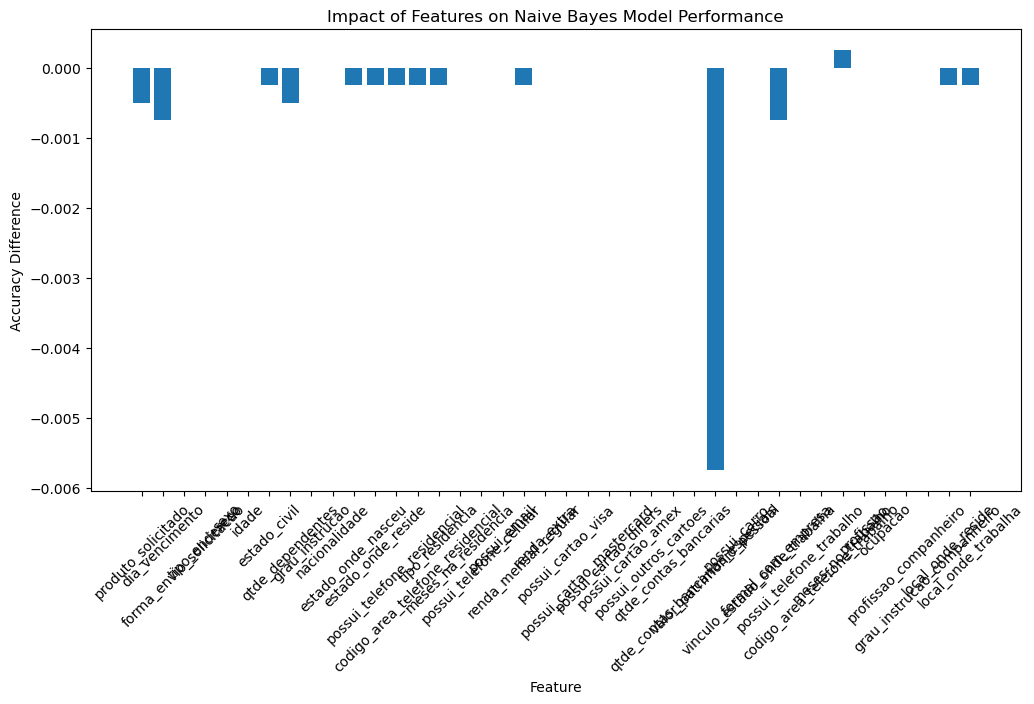
\includegraphics{C:/Users/carol/OneDrive/Documentos/GitHub/Introduction-to-Machine-Learning-EEL891/Trabalho 1 - Classificador/Data Analysis/features-originais.png}
\caption{Gráfico com todas as features originais}
\end{figure}

Após a remoção de `valor\_patrimonio\_pessoal', a acurácia subiu para
51.05\% e a função \texttt{compare\_feature\_impact} sugeriu a remoção
das features `renda\_mensal\_regular' e `renda\_extra'. O parâmetro de
diferença de acurácias menor ou igual a -0.005 provou ser muito
eficiente pois, a cada remoção, o gráfico aparentava se estabilizar
ainda mais. A figura abaixo apresenta o gráfico depois da remoção das
categorias de renda.

\begin{figure}
\centering
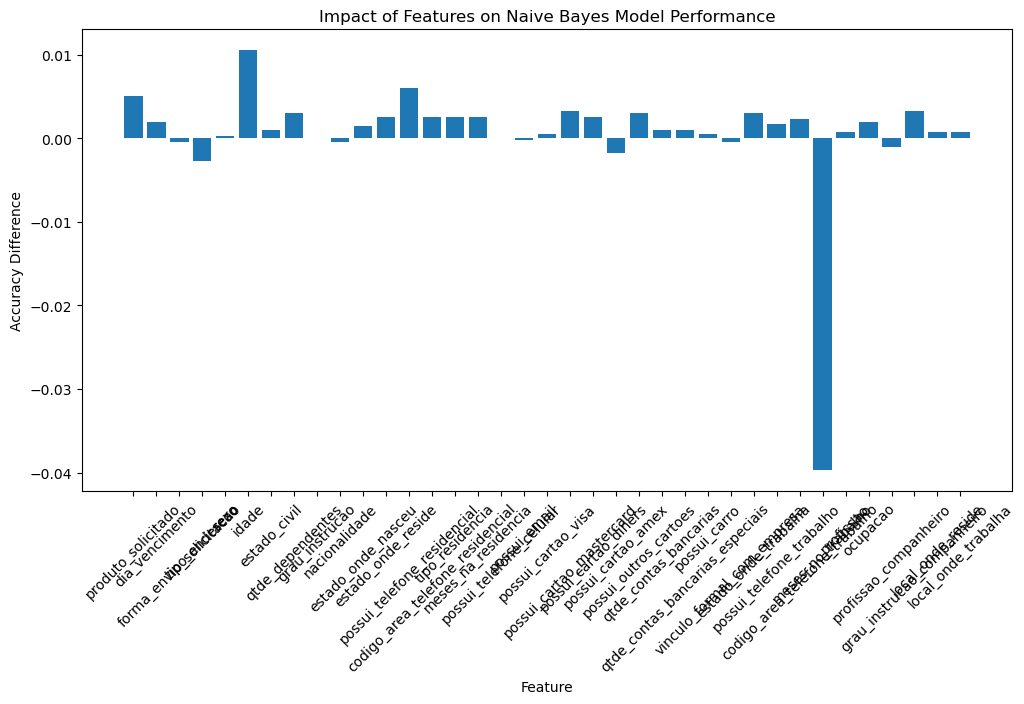
\includegraphics{C:/Users/carol/OneDrive/Documentos/GitHub/Introduction-to-Machine-Learning-EEL891/Trabalho 1 - Classificador/Data Analysis/remocao_de_rendas.png}
\caption{Gráfico sem `renda\_mensal\_regular' e `renda\_extra'}
\end{figure}

Com isso, torna-se óbvia a necessidade da remoção de
`meses\_no\_trabalho'. A nova acurácia sobe para 56.25\%, mas ainda
variando entre 54.9\% até 57.7\%. A seguir, o gráfico de impacto após
esse passo.

\begin{figure}
\centering
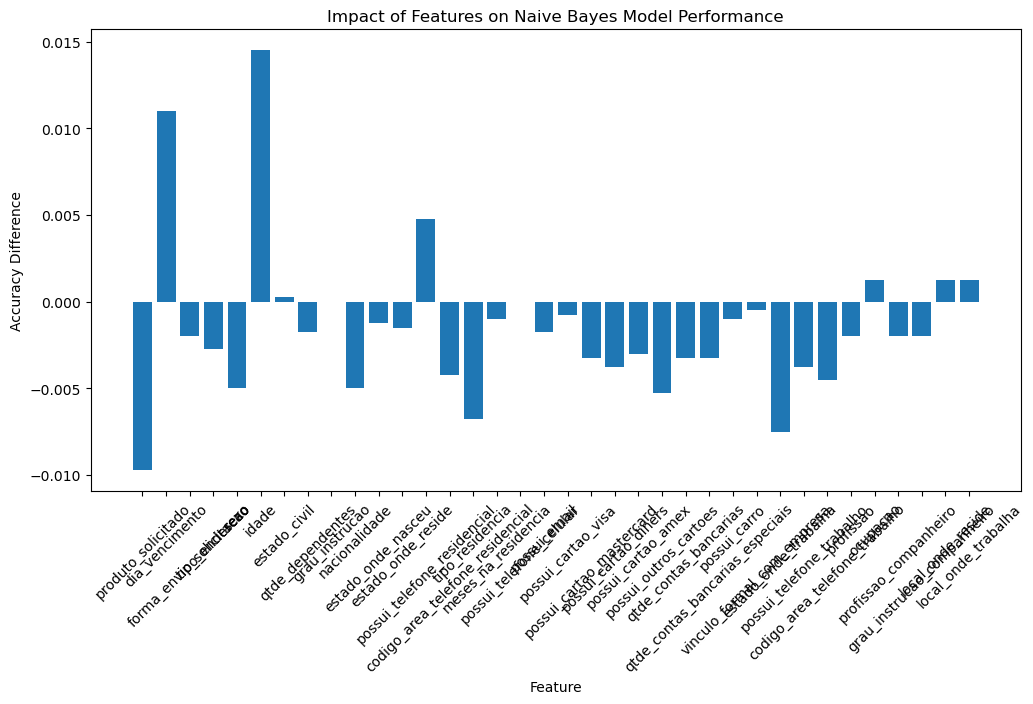
\includegraphics{C:/Users/carol/OneDrive/Documentos/GitHub/Introduction-to-Machine-Learning-EEL891/Trabalho 1 - Classificador/Data Analysis/remocao-meses-trab.png}
\caption{Gráfico sem `meses\_no\_trabalho'}
\end{figure}

Seguindo com a análise, a função sugere a remoção de 5 features, mas foi
decidido que seriam removidas apenas as duas com diferença de acurácia
de maiores módulos. Nesse caso, foram as categorias
`produto\_solicitado' e `estado\_onde\_trabalha'. A acurácia subiu para
uma média de 56.5\%, e o gráfico apresentou extrema estabilização entre
as variáveis.

\begin{figure}
\centering
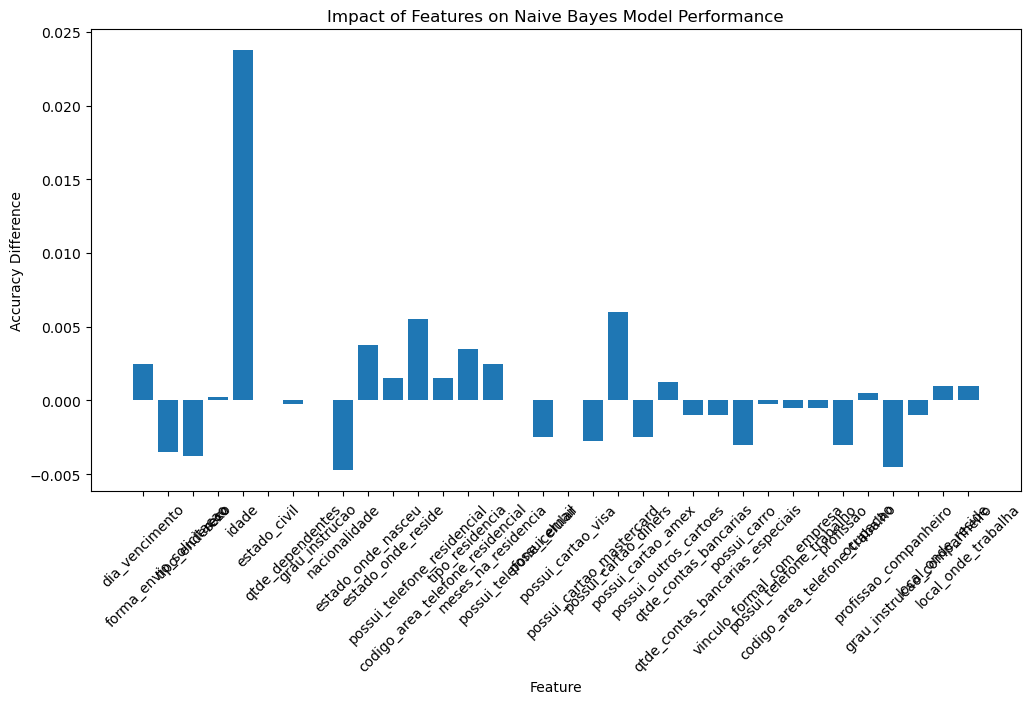
\includegraphics{C:/Users/carol/OneDrive/Documentos/GitHub/Introduction-to-Machine-Learning-EEL891/Trabalho 1 - Classificador/Data Analysis/produtosol-estadotrab.png}
\caption{Gráfico sem `produto\_solicitado' e `estado\_onde\_trabalha'}
\end{figure}

\hypertarget{funuxe7uxe3o-generate_bar_charts}{%
\subsubsection{Função
generate\_bar\_charts}\label{funuxe7uxe3o-generate_bar_charts}}

A função \texttt{generate\_bar\_charts(df)} é responsável por gerar
gráficos de barras para todas as colunas do DataFrame fornecido. Ela
itera sobre cada coluna e verifica o tipo de dados. Se a coluna for do
tipo categórico, a função conta o número de ocorrências de cada valor na
coluna e cria um gráfico de barras para visualizar a distribuição dos
dados.

O dicionário \texttt{bar\_charts} é criado para armazenar os gráficos de
barras de cada coluna. Cada gráfico é plotado usando a biblioteca
\texttt{matplotlib.pyplot}.

A segunda etapa do Pré-Processamento de Dados consiste na análise dos
gráficos gerados, para avaliar se todas as variáveis estão de acordo com
o modelo. Foi notado que as variáveis `possui\_outros\_cartoes',
`possui\_telefone\_celular' e `grau\_instrucao' deveriam ser removidas.

\begin{figure}
\centering
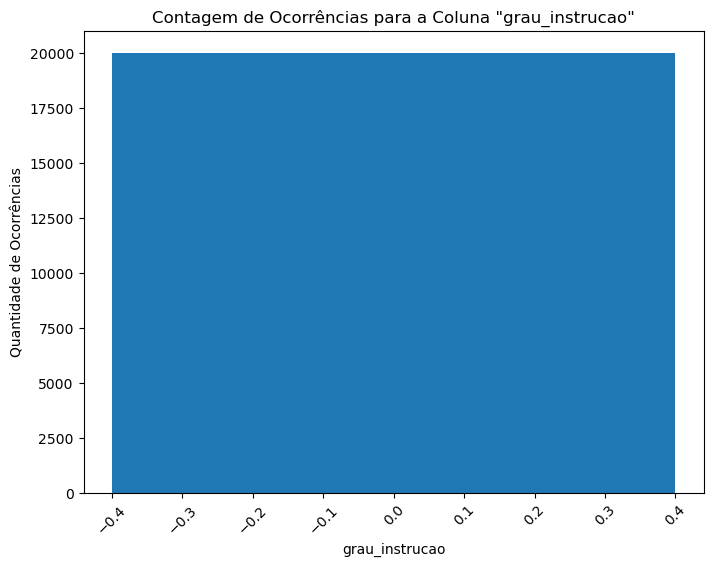
\includegraphics{C:/Users/carol/OneDrive/Documentos/GitHub/Introduction-to-Machine-Learning-EEL891/Trabalho 1 - Classificador/Data Analysis/grauinstrucao.png}
\caption{Gráfico de `grau\_instrucao'}
\end{figure}

\begin{figure}
\centering
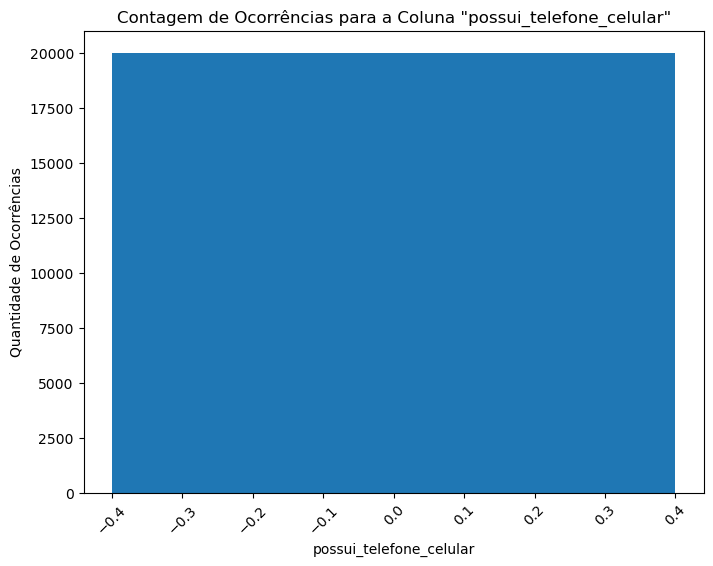
\includegraphics{C:/Users/carol/OneDrive/Documentos/GitHub/Introduction-to-Machine-Learning-EEL891/Trabalho 1 - Classificador/Data Analysis/telefonecelular.png}
\caption{Gráfico de `possui\_telefone\_celular'}
\end{figure}

\begin{figure}
\centering
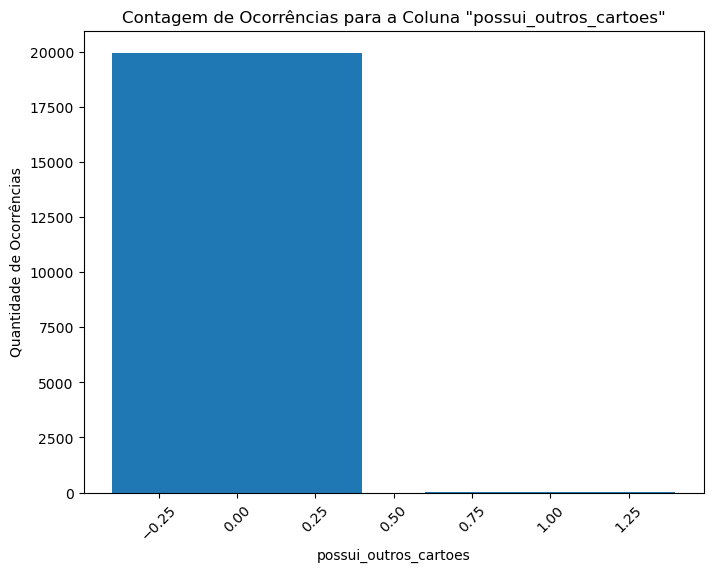
\includegraphics{C:/Users/carol/OneDrive/Documentos/GitHub/Introduction-to-Machine-Learning-EEL891/Trabalho 1 - Classificador/Data Analysis/possuioutroscartoes.png}
\caption{Gráfico de `possui\_outros\_cartoes'}
\end{figure}

Após essa etapa, foi observa uma acurácia média de 56.67\% e um gráfico
de impacto das variaveis no seguinte formato, sem muitas mudanças:

\begin{figure}
\centering
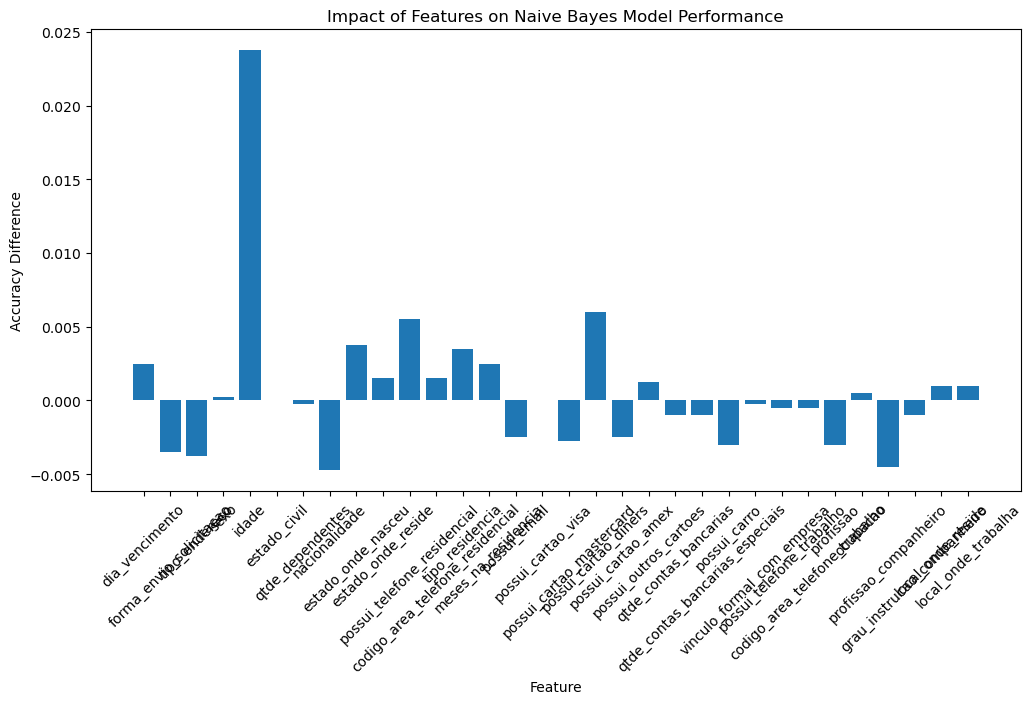
\includegraphics{C:/Users/carol/OneDrive/Documentos/GitHub/Introduction-to-Machine-Learning-EEL891/Trabalho 1 - Classificador/Data Analysis/graficofuncao2.png}
\caption{Gráfico de impacto}
\end{figure}

    \begin{tcolorbox}[breakable, size=fbox, boxrule=1pt, pad at break*=1mm,colback=cellbackground, colframe=cellborder]
\prompt{In}{incolor}{ }{\boxspacing}
\begin{Verbatim}[commandchars=\\\{\}]
\PY{k+kn}{import} \PY{n+nn}{matplotlib}\PY{n+nn}{.}\PY{n+nn}{pyplot} \PY{k}{as} \PY{n+nn}{plt}
\PY{k+kn}{from} \PY{n+nn}{sklearn}\PY{n+nn}{.}\PY{n+nn}{model\PYZus{}selection} \PY{k+kn}{import} \PY{n}{train\PYZus{}test\PYZus{}split}
\PY{k+kn}{from} \PY{n+nn}{sklearn}\PY{n+nn}{.}\PY{n+nn}{metrics} \PY{k+kn}{import} \PY{n}{accuracy\PYZus{}score}


\PY{k}{def} \PY{n+nf}{compare\PYZus{}feature\PYZus{}impact}\PY{p}{(}\PY{n}{df}\PY{p}{,} \PY{n}{target\PYZus{}column}\PY{p}{)}\PY{p}{:}
    \PY{c+c1}{\PYZsh{} Prepare the feature matrix (X) and target variable (y)}
    \PY{n}{X} \PY{o}{=} \PY{n}{df}\PY{o}{.}\PY{n}{drop}\PY{p}{(}\PY{n}{target\PYZus{}column}\PY{p}{,} \PY{n}{axis}\PY{o}{=}\PY{l+m+mi}{1}\PY{p}{)}
    \PY{n}{y} \PY{o}{=} \PY{n}{df}\PY{p}{[}\PY{n}{target\PYZus{}column}\PY{p}{]}

    \PY{c+c1}{\PYZsh{} Split the dataset into training and testing sets}
    \PY{n}{X\PYZus{}train}\PY{p}{,} \PY{n}{X\PYZus{}test}\PY{p}{,} \PY{n}{y\PYZus{}train}\PY{p}{,} \PY{n}{y\PYZus{}test} \PY{o}{=} \PY{n}{train\PYZus{}test\PYZus{}split}\PY{p}{(}\PY{n}{X}\PY{p}{,} \PY{n}{y}\PY{p}{,} \PY{n}{test\PYZus{}size}\PY{o}{=}\PY{l+m+mf}{0.2}\PY{p}{,} \PY{n}{random\PYZus{}state}\PY{o}{=}\PY{l+m+mi}{42}\PY{p}{)}

    \PY{c+c1}{\PYZsh{} Create and train the Naive Bayes model with all features}
    \PY{n}{naive\PYZus{}bayes\PYZus{}model\PYZus{}with\PYZus{}all\PYZus{}features} \PY{o}{=} \PY{n}{GaussianNB}\PY{p}{(}\PY{p}{)}
    \PY{n}{naive\PYZus{}bayes\PYZus{}model\PYZus{}with\PYZus{}all\PYZus{}features}\PY{o}{.}\PY{n}{fit}\PY{p}{(}\PY{n}{X\PYZus{}train}\PY{p}{,} \PY{n}{y\PYZus{}train}\PY{p}{)}

    \PY{c+c1}{\PYZsh{} Get the baseline accuracy with all features included}
    \PY{n}{y\PYZus{}pred\PYZus{}with\PYZus{}all\PYZus{}features} \PY{o}{=} \PY{n}{naive\PYZus{}bayes\PYZus{}model\PYZus{}with\PYZus{}all\PYZus{}features}\PY{o}{.}\PY{n}{predict}\PY{p}{(}\PY{n}{X\PYZus{}test}\PY{p}{)}
    \PY{n}{baseline\PYZus{}accuracy} \PY{o}{=} \PY{n}{accuracy\PYZus{}score}\PY{p}{(}\PY{n}{y\PYZus{}test}\PY{p}{,} \PY{n}{y\PYZus{}pred\PYZus{}with\PYZus{}all\PYZus{}features}\PY{p}{)}

    \PY{c+c1}{\PYZsh{} Create a dictionary to store the feature names and their corresponding accuracy differences}
    \PY{n}{feature\PYZus{}impact} \PY{o}{=} \PY{p}{\PYZob{}}\PY{p}{\PYZcb{}}

    \PY{c+c1}{\PYZsh{} Create an empty list to store features with a small accuracy difference}
    \PY{n}{features\PYZus{}to\PYZus{}remove} \PY{o}{=} \PY{p}{[}\PY{p}{]}

    \PY{c+c1}{\PYZsh{} Iterate over each feature and compare the model performance with and without the feature}
    \PY{k}{for} \PY{n}{feature} \PY{o+ow}{in} \PY{n}{X}\PY{o}{.}\PY{n}{columns}\PY{p}{:}
        \PY{c+c1}{\PYZsh{} Train the Naive Bayes model without the current feature}
        \PY{n}{X\PYZus{}train\PYZus{}without\PYZus{}feature} \PY{o}{=} \PY{n}{X\PYZus{}train}\PY{o}{.}\PY{n}{drop}\PY{p}{(}\PY{n}{feature}\PY{p}{,} \PY{n}{axis}\PY{o}{=}\PY{l+m+mi}{1}\PY{p}{)}
        \PY{n}{X\PYZus{}test\PYZus{}without\PYZus{}feature} \PY{o}{=} \PY{n}{X\PYZus{}test}\PY{o}{.}\PY{n}{drop}\PY{p}{(}\PY{n}{feature}\PY{p}{,} \PY{n}{axis}\PY{o}{=}\PY{l+m+mi}{1}\PY{p}{)}

        \PY{n}{naive\PYZus{}bayes\PYZus{}model\PYZus{}without\PYZus{}feature} \PY{o}{=} \PY{n}{GaussianNB}\PY{p}{(}\PY{p}{)}
        \PY{n}{naive\PYZus{}bayes\PYZus{}model\PYZus{}without\PYZus{}feature}\PY{o}{.}\PY{n}{fit}\PY{p}{(}\PY{n}{X\PYZus{}train\PYZus{}without\PYZus{}feature}\PY{p}{,} \PY{n}{y\PYZus{}train}\PY{p}{)}

        \PY{c+c1}{\PYZsh{} Get the accuracy without the feature}
        \PY{n}{y\PYZus{}pred\PYZus{}without\PYZus{}feature} \PY{o}{=} \PY{n}{naive\PYZus{}bayes\PYZus{}model\PYZus{}without\PYZus{}feature}\PY{o}{.}\PY{n}{predict}\PY{p}{(}\PY{n}{X\PYZus{}test\PYZus{}without\PYZus{}feature}\PY{p}{)}
        \PY{n}{accuracy\PYZus{}without\PYZus{}feature} \PY{o}{=} \PY{n}{accuracy\PYZus{}score}\PY{p}{(}\PY{n}{y\PYZus{}test}\PY{p}{,} \PY{n}{y\PYZus{}pred\PYZus{}without\PYZus{}feature}\PY{p}{)}

        \PY{c+c1}{\PYZsh{} Calculate the accuracy difference compared to the baseline}
        \PY{n}{feature\PYZus{}impact}\PY{p}{[}\PY{n}{feature}\PY{p}{]} \PY{o}{=} \PY{n}{baseline\PYZus{}accuracy} \PY{o}{\PYZhy{}} \PY{n}{accuracy\PYZus{}without\PYZus{}feature}

        \PY{c+c1}{\PYZsh{} Check if the accuracy difference is smaller than \PYZhy{}0.005 and add the feature to the list}
        \PY{k}{if} \PY{n}{feature\PYZus{}impact}\PY{p}{[}\PY{n}{feature}\PY{p}{]} \PY{o}{\PYZlt{}}\PY{o}{=} \PY{o}{\PYZhy{}}\PY{l+m+mf}{0.005}\PY{p}{:}
            \PY{n}{features\PYZus{}to\PYZus{}remove}\PY{o}{.}\PY{n}{append}\PY{p}{(}\PY{n}{feature}\PY{p}{)}
    \PY{n}{features\PYZus{}to\PYZus{}remove}\PY{o}{.}\PY{n}{sort}\PY{p}{(}\PY{n}{key}\PY{o}{=}\PY{k}{lambda} \PY{n}{x}\PY{p}{:} \PY{n}{feature\PYZus{}impact}\PY{p}{[}\PY{n}{x}\PY{p}{]}\PY{p}{)}    


    \PY{c+c1}{\PYZsh{} Create a bar plot showing the impact of each feature on the model\PYZsq{}s performance}
    \PY{n}{plt}\PY{o}{.}\PY{n}{figure}\PY{p}{(}\PY{n}{figsize}\PY{o}{=}\PY{p}{(}\PY{l+m+mi}{12}\PY{p}{,} \PY{l+m+mi}{6}\PY{p}{)}\PY{p}{)}
    \PY{n}{plt}\PY{o}{.}\PY{n}{bar}\PY{p}{(}\PY{n}{feature\PYZus{}impact}\PY{o}{.}\PY{n}{keys}\PY{p}{(}\PY{p}{)}\PY{p}{,} \PY{n}{feature\PYZus{}impact}\PY{o}{.}\PY{n}{values}\PY{p}{(}\PY{p}{)}\PY{p}{)}
    \PY{n}{plt}\PY{o}{.}\PY{n}{xlabel}\PY{p}{(}\PY{l+s+s1}{\PYZsq{}}\PY{l+s+s1}{Feature}\PY{l+s+s1}{\PYZsq{}}\PY{p}{)}
    \PY{n}{plt}\PY{o}{.}\PY{n}{ylabel}\PY{p}{(}\PY{l+s+s1}{\PYZsq{}}\PY{l+s+s1}{Accuracy Difference}\PY{l+s+s1}{\PYZsq{}}\PY{p}{)}
    \PY{n}{plt}\PY{o}{.}\PY{n}{title}\PY{p}{(}\PY{l+s+s1}{\PYZsq{}}\PY{l+s+s1}{Impact of Features on Naive Bayes Model Performance}\PY{l+s+s1}{\PYZsq{}}\PY{p}{)}
    \PY{n}{plt}\PY{o}{.}\PY{n}{xticks}\PY{p}{(}\PY{n}{rotation}\PY{o}{=}\PY{l+m+mi}{45}\PY{p}{)}
    \PY{n}{plt}\PY{o}{.}\PY{n}{show}\PY{p}{(}\PY{p}{)}

    \PY{c+c1}{\PYZsh{} Print the list of features with accuracy difference smaller than \PYZhy{}0.005}
    \PY{n+nb}{print}\PY{p}{(}\PY{l+s+s2}{\PYZdq{}}\PY{l+s+s2}{Features to Remove:}\PY{l+s+s2}{\PYZdq{}}\PY{p}{)}
    \PY{n+nb}{print}\PY{p}{(}\PY{n}{features\PYZus{}to\PYZus{}remove}\PY{p}{)}




\PY{n}{compare\PYZus{}feature\PYZus{}impact}\PY{p}{(}\PY{n}{df\PYZus{}train}\PY{p}{,} \PY{l+s+s1}{\PYZsq{}}\PY{l+s+s1}{inadimplente}\PY{l+s+s1}{\PYZsq{}}\PY{p}{)}
\end{Verbatim}
\end{tcolorbox}

    \begin{tcolorbox}[breakable, size=fbox, boxrule=1pt, pad at break*=1mm,colback=cellbackground, colframe=cellborder]
\prompt{In}{incolor}{ }{\boxspacing}
\begin{Verbatim}[commandchars=\\\{\}]
\PY{k+kn}{import} \PY{n+nn}{matplotlib}\PY{n+nn}{.}\PY{n+nn}{pyplot} \PY{k}{as} \PY{n+nn}{plt}

\PY{k}{def} \PY{n+nf}{generate\PYZus{}bar\PYZus{}charts}\PY{p}{(}\PY{n}{df}\PY{p}{)}\PY{p}{:}
    \PY{c+c1}{\PYZsh{} Cria um dicionário para armazenar os gráficos de barras de cada coluna}
    \PY{n}{bar\PYZus{}charts} \PY{o}{=} \PY{p}{\PYZob{}}\PY{p}{\PYZcb{}}

    \PY{c+c1}{\PYZsh{} Itera sobre todas as colunas do DataFrame}
    \PY{k}{for} \PY{n}{column} \PY{o+ow}{in} \PY{n}{df}\PY{o}{.}\PY{n}{columns}\PY{p}{:}
        \PY{c+c1}{\PYZsh{} Verifica o tipo da coluna (objeto é tratado como categórico)}
        
        \PY{c+c1}{\PYZsh{} Conta o número de ocorrências de cada valor na coluna}
        \PY{n}{value\PYZus{}counts} \PY{o}{=} \PY{n}{df}\PY{p}{[}\PY{n}{column}\PY{p}{]}\PY{o}{.}\PY{n}{value\PYZus{}counts}\PY{p}{(}\PY{p}{)}

        \PY{c+c1}{\PYZsh{} Cria um gráfico de barras}
        \PY{n}{plt}\PY{o}{.}\PY{n}{figure}\PY{p}{(}\PY{n}{figsize}\PY{o}{=}\PY{p}{(}\PY{l+m+mi}{8}\PY{p}{,} \PY{l+m+mi}{6}\PY{p}{)}\PY{p}{)}
        \PY{n}{plt}\PY{o}{.}\PY{n}{bar}\PY{p}{(}\PY{n}{value\PYZus{}counts}\PY{o}{.}\PY{n}{index}\PY{p}{,} \PY{n}{value\PYZus{}counts}\PY{o}{.}\PY{n}{values}\PY{p}{)}
        \PY{n}{plt}\PY{o}{.}\PY{n}{xlabel}\PY{p}{(}\PY{n}{column}\PY{p}{)}
        \PY{n}{plt}\PY{o}{.}\PY{n}{ylabel}\PY{p}{(}\PY{l+s+s1}{\PYZsq{}}\PY{l+s+s1}{Quantidade de Ocorrências}\PY{l+s+s1}{\PYZsq{}}\PY{p}{)}
        \PY{n}{plt}\PY{o}{.}\PY{n}{title}\PY{p}{(}\PY{l+s+sa}{f}\PY{l+s+s1}{\PYZsq{}}\PY{l+s+s1}{Contagem de Ocorrências para a Coluna }\PY{l+s+s1}{\PYZdq{}}\PY{l+s+si}{\PYZob{}}\PY{n}{column}\PY{l+s+si}{\PYZcb{}}\PY{l+s+s1}{\PYZdq{}}\PY{l+s+s1}{\PYZsq{}}\PY{p}{)}
        \PY{n}{plt}\PY{o}{.}\PY{n}{xticks}\PY{p}{(}\PY{n}{rotation}\PY{o}{=}\PY{l+m+mi}{45}\PY{p}{)}
        \PY{n}{plt}\PY{o}{.}\PY{n}{show}\PY{p}{(}\PY{p}{)}

        \PY{c+c1}{\PYZsh{} Adiciona o gráfico ao dicionário}
        \PY{n}{bar\PYZus{}charts}\PY{p}{[}\PY{n}{column}\PY{p}{]} \PY{o}{=} \PY{n}{plt}

    \PY{k}{return} \PY{n}{bar\PYZus{}charts}

\PY{n}{generate\PYZus{}bar\PYZus{}charts}\PY{p}{(}\PY{n}{df\PYZus{}train}\PY{p}{)}
\end{Verbatim}
\end{tcolorbox}

    \hypertarget{resultados}{%
\subsection{Resultados}\label{resultados}}

Seção utilizada para salvar os resultados num arquivo
``predictions.csv''.

    \begin{tcolorbox}[breakable, size=fbox, boxrule=1pt, pad at break*=1mm,colback=cellbackground, colframe=cellborder]
\prompt{In}{incolor}{ }{\boxspacing}
\begin{Verbatim}[commandchars=\\\{\}]
\PY{n}{df\PYZus{}test} \PY{o}{=} \PY{n}{pd}\PY{o}{.}\PY{n}{read\PYZus{}csv}\PY{p}{(}\PY{l+s+s1}{\PYZsq{}}\PY{l+s+s1}{Dataset/conjunto\PYZus{}de\PYZus{}teste.csv}\PY{l+s+s1}{\PYZsq{}}\PY{p}{)}

\PY{n}{prediction\PYZus{}file} \PY{o}{=} \PY{n}{pd}\PY{o}{.}\PY{n}{DataFrame}\PY{p}{(}\PY{n}{predictions}\PY{p}{,} \PY{n}{columns}\PY{o}{=}\PY{p}{[}\PY{l+s+s1}{\PYZsq{}}\PY{l+s+s1}{inadimplente}\PY{l+s+s1}{\PYZsq{}}\PY{p}{]}\PY{p}{)}
\PY{n}{prediction\PYZus{}file} \PY{o}{=} \PY{n}{pd}\PY{o}{.}\PY{n}{concat}\PY{p}{(}\PY{p}{[}\PY{n}{df\PYZus{}test}\PY{p}{[}\PY{l+s+s1}{\PYZsq{}}\PY{l+s+s1}{id\PYZus{}solicitante}\PY{l+s+s1}{\PYZsq{}}\PY{p}{]}\PY{p}{,} \PY{n}{prediction\PYZus{}file}\PY{p}{]}\PY{p}{,} \PY{n}{axis}\PY{o}{=}\PY{l+m+mi}{1}\PY{p}{)}
\PY{n}{prediction\PYZus{}file} \PY{o}{=} \PY{n}{prediction\PYZus{}file}\PY{o}{.}\PY{n}{to\PYZus{}csv}\PY{p}{(}\PY{l+s+s1}{\PYZsq{}}\PY{l+s+s1}{results/predictions.csv}\PY{l+s+s1}{\PYZsq{}}\PY{p}{,} \PY{n}{index}\PY{o}{=}\PY{k+kc}{False}\PY{p}{)}


\PY{n}{prediction\PYZus{}file} \PY{o}{=} \PY{n}{pd}\PY{o}{.}\PY{n}{read\PYZus{}csv}\PY{p}{(}\PY{l+s+s1}{\PYZsq{}}\PY{l+s+s1}{results/predictions.csv}\PY{l+s+s1}{\PYZsq{}}\PY{p}{)}
\PY{n}{prediction\PYZus{}file}\PY{o}{.}\PY{n}{shape}
\end{Verbatim}
\end{tcolorbox}


    % Add a bibliography block to the postdoc
    
    
    
\end{document}
